% !TeX encoding = UTF-8

% 载入 SJTUThesis 模版
\documentclass[type=master, openright]{sjtuthesis}
% 选项
%   type=[doctor|master|bachelor],     % 可选(默认:master),论文类型
%   zihao=[-4|5],                      % 可选(默认:-4),正文字号大小
%   lang=[zh|en|de|ja],                % 可选(默认:zh),论文的主要语言
%   review,                            % 可选(默认:关闭),盲审模式
%   [twoside|oneside],                 % 可选(默认:twoside),双页或单页边距模式
%   [openright|openany],               % 可选(默认:openright),奇数页或任意页开始新章
%   math-style=[ISO|TeX],              % 可选 (默认:ISO),数学符号样式

% 论文基本配置,加载宏包等全局配置
% !TEX root = ./main.tex

\sjtusetup{
  %
  %******************************
  % 注意:
  %   1. 配置里面不要出现空行
  %   2. 不需要的配置信息可以删除
  %******************************
  %
  % 信息录入
  %
  info = {%
    %
    % 标题
    %
    zh / title           = {高效时序图处理系统的设计与实现},
    en / title           = {Design and implementation of efficient Temporal Graph Processing system},
    %
    % 标题页标题
    %   可使用“\\”命令手动控制换行
    %
    % zh / display-title   = {上海交通大学学位论文\\ \LaTeX{} 模板示例文档},
    % en / display-title   = {A Sample Document \\ for \LaTeX-based SJTU Thesis Template},
    %
    % 关键词
    %
    zh / keywords        = {时序图,图处理,图查询,图分析},
    en / keywords        = {Temporal Graph, Graph Processing, Graph Query, Graph Analysis},
    %
    % 姓名
    %
    zh / author          = {石\quad{}林},
    en / author          = {Lin Shi},
    %
    % 指导教师
    %
    zh / supervisor      = {陈榕\ 教授},
    en / supervisor      = {Prof. Rong Chen},
    %
    % 学号
    %
    id              = {121037910049},
    %
    % 学位
    %
    zh / degree          = {专业学位硕士},
    en / degree          = {Master of Engineering},
    %
    % 专业
    %
    zh / major           = {电子信息},
    en / major           = {Electronic Information},
    %
    % 所属院系
    %
    zh / department      = {电子信息与电气工程学院},
    en / department      = {School of Electronic Information and Electrical Engineering},
    %
    % 答辩日期
    %   使用 ISO 格式 (yyyy-mm-dd);默认为当前时间
    %
    % date                 = {2023-05-18},
    %
    % 标题页显示日期
    %   覆盖对应标题页的日期显示,原样输出
    %
    % zh / display-date    = {2023 年 5 月},
  },
  %
  % 风格设置
  %
  style = {%
    %
    % 论文标题页 logo 颜色 (red/blue/black)
    %
    % title-logo-color = black,
  },
  %
  % 名称设置
  %
  name = {
    % bib             = {References},
    % ack             = {谢\hspace{\ccwd}辞},
    % achv            = {攻读学位期间完成的论文},
  },
}

% 使用 BibLaTeX 处理参考文献
%   biblatex-gb7714-2015 常用选项
%     gbnamefmt=lowercase     姓名大小写由输入信息确定
%     gbpub=false             禁用出版信息缺失处理
\usepackage[backend=biber,style=gb7714-2015]{biblatex}
% 文献表字体
% \renewcommand{\bibfont}{\zihao{5}\fixedlineskip{15.6bp}}
% 文献表条目间的间距
\setlength{\bibitemsep}{0pt}
% 导入参考文献数据库
\addbibresource{refs.bib}

% 脚注格式
\usepackage[perpage,bottom,hang]{footmisc}

% 定义图片文件目录与扩展名
\graphicspath{{figures/}}
\DeclareGraphicsExtensions{.pdf,.eps,.png,.jpg,.jpeg}

% 确定浮动对象的位置,可以使用 [H],强制将浮动对象放到这里(可能效果很差)
% \usepackage{float}

% 固定宽度的表格
% \usepackage{tabularx}

% 使用三线表:toprule,midrule,bottomrule。
\usepackage{booktabs}

\usepackage{pifont}

% 表格中支持跨行
\usepackage{multirow}

% 表格中数字按小数点对齐
\usepackage{dcolumn}
\newcolumntype{d}[1]{D{.}{.}{#1}}

% 使用长表格
\usepackage{longtable}

% 附带脚注的表格
\usepackage{threeparttable}

% 附带脚注的长表格
\usepackage{threeparttablex}

% 算法环境宏包
\usepackage[ruled,vlined,linesnumbered]{algorithm2e}
% \usepackage{algorithm, algorithmicx, algpseudocode}

% 代码环境宏包
\usepackage{listings}
\lstdefinestyle{lstStyleCode}{%
  aboveskip         = \medskipamount,
  belowskip         = \medskipamount,
  basicstyle        = \ttfamily\zihao{6},
  commentstyle      = \slshape\color{black!60},
  stringstyle       = \color{green!40!black!100},
  keywordstyle      = \bfseries\color{blue!50!black},
  extendedchars     = false,
  upquote           = true,
  tabsize           = 2,
  showstringspaces  = false,
  xleftmargin       = 1em,
  xrightmargin      = 1em,
  breaklines        = false,
  framexleftmargin  = 1em,
  framexrightmargin = 1em,
  backgroundcolor   = \color{gray!10},
  columns           = flexible,
  keepspaces        = true,
  texcl             = true,
  mathescape        = true
}
\lstnewenvironment{codeblock}[1][]{%
  \lstset{style=lstStyleCode,#1}}{}

% 直立体数学符号
\providecommand{\dd}{\mathop{}\!\mathrm{d}}
\providecommand{\ee}{\mathrm{e}}
\providecommand{\ii}{\mathrm{i}}
\providecommand{\jj}{\mathrm{j}}

% 国际单位制宏包
\usepackage{siunitx}

% 定理环境宏包
\usepackage{ntheorem}
% \usepackage{amsthm}

% 绘图宏包
\usepackage{tikz}
\usetikzlibrary{arrows.meta, shapes.geometric}

% 一些文档中用到的 logo
\usepackage{hologo}
\providecommand{\XeTeX}{\hologo{XeTeX}}
\providecommand{\BibLaTeX}{\textsc{Bib}\LaTeX}

% 借用 ltxdoc 里面的几个命令方便写文档
\DeclareRobustCommand\cs[1]{\texttt{\char`\\#1}}
\providecommand\pkg[1]{{\sffamily#1}}

% hyperref 宏包在最后调用
\usepackage{hyperref}

% E-mail
\providecommand{\email}[1]{\href{mailto:#1}{\urlstyle{tt}\nolinkurl{#1}}}

\newcommand{\sys}{\textsc{TempGraph}}
\newcommand{\store}{SegCSR/TS}
\newcommand{\newstore}{SegCSR}
\newcommand{\todo}[1]{\textcolor{red}{TODO: #1}\PackageWarning{TODO:}{#1!}}

\begin{document}

%TC:ignore

% 标题页
\maketitle

% 原创性声明及使用授权书
\copyrightpage
% 插入外置原创性声明及使用授权书
% 此时必须在导言区使用 \usepackage{pdfpages}
% \copyrightpage[scans/sample-copyright.pdf]

% 前置部分
\frontmatter

% 摘要
% !TEX root = ../main.tex

\begin{abstract}[zh]
越来越多的图状结构数据包含时序信息,这些时序信息描述了实体和关系的生命周期,时序图是表示包含时序信息的图状结构数据的常用模型。
时序图的更新、时序图查询和时序图分析是三类最为重要的时序图处理任务。
时序图查询可以是面向时序图的特定版本(包括最新版本和历史版本)的基于图拓扑的查询,也可以是基于时序图中顶点/边的生命周期信息的查询。
时序图分析任务同样既可以是在时序图的特定版本上的普通图分析任务,也可以使用时序图的生命周期信息运行更为复杂的图分析算法。

时序RDF图、时序超图和时序属性图是定义时序图结构的三大模型,但面向时序RDF图和时序超图的时序图查询并不是热点研究方向,相关系统研究工作不多,且性能难以令人满意。
在线图分析系统通常使用时序属性图模型作为其数据模型,与离线图分析系统相比,这类系统同时实现了图的更新和分析,且能够在图更新完成后的很短时间内对其进行分析,大大提高了图分析的时效性,但这要以大幅牺牲图分析性能为代价。

针对上述问题,本文设计并实现了一个高效的时序图处理系统\sys,它由时序图查询和时序图分析两大模块组成。
系统的时序图查询模块同时支持时序RDF图和时序超图的高效查询,它使用了基于RDMA的分布式键值存储辅以分布式排序数组的存储结构,键值存储使用了直接索引和间接索引相结合的设计,在实现了高效的
拓扑查询和时间条件查询的同时,减少了时序数据存储的内存使用。
系统的时序图分析模块实现了图的事务化更新和实时的第一类时序图分析,它使用了一个高效可更新的时序属性图存储结构\newstore,并使用了一种粗粒度的多版本并发控制机制来减少时序数据带来的内存使用和图分析时的额外计算开销。

本文从多个角度对\sys 进行了全面的性能评测,测试结果表明,与图数据库NebulaGraph和Neo4j相比,\sys 的时序图查询都有一个数量级以上的性能提升,\sys 的图分析性能是目前最先进的在线图分析系统LiveGraph的1.4\textasciitilde 4.4倍。

\end{abstract}

\begin{abstract}[en]
More and more graph-structured data contain temporal information, which describes the lifespan of entities and relationships. 
Temporal graph is a commonly used model to represent graph-structured data with temporal information. 
The three most important temporal graph processing tasks are temporal graph updating, temporal graph query, and temporal graph analysis.
A temporal graph query can be either a topology-based query on a specific version (the latest or historical version) of the temporal graph, or a query based on the lifespan information of vertices/edges in the temporal graph. 
A temporal graph analysis task can be either a regular graph analysis task on a specific version of the temporal graph, or a more complex graph analysis algorithm that utilizes the lifespan information of the temporal graph.

The three major models defining the structure of a temporal graph are the temporal RDF graph, the temporal hypergraph, and the temporal property graph.
Temporal graph query on the temporal RDF graph and hypergraph is not a hot research topic, with limited relevant system research and unsatisfactory system performance. 
Online graph analysis systems typically use temporal property graph model as their data model. Compared to offline graph analysis systems, these systems can achieve both graph updating and analysis, enabling them to analyze the graph shortly after it is updated, greatly improving the freshness of graph analysis. 
However, this comes at the cost of sacrificing graph analysis performance significantly.

To address the above issues, this paper designs and implements an efficient temporal graph processing system called \sys, which consists of two modules: temporal graph query and analysis. 
The temporal graph query module of the system supports efficient query for both temporal RDF graph and hypergraph. 
Its storage structure is a distributed key-value storage, supplemented by distributed sorted arrays based on RDMA.
The key-value storage adopts a design that combines direct and indirect indexing, which achieves efficient topological and time-condition queries while reducing the memory usage for storing temporal data. 
The temporal graph analysis module of the system implements transactional graph updating and real-time type-1 temporal graph analysis. 
It utilizes an efficient updatable temporal property graph storage structure called \newstore, and a coarse-grained multi-version concurrency control mechanism to reduce memory usage and additional computational overhead during graph analysis caused by temporal data.

Comprehensive performance evaluations of \sys are conducted from multiple perspectives in this paper.
The evaluation results demonstrate that compared to graph databases NebulaGraph and Neo4j, \sys \ achieves temporal graph query performance improvements of over an order of magnitude, and its graph analysis performance is 1.4\textasciitilde 4.4 times better than that of the state-of-the-art online graph analysis system LiveGraph.
\end{abstract}


% 目录
\tableofcontents
% 插图索引
\listoffigures*
% 表格索引
\listoftables*
% 算法索引
\listofalgorithms*

%TC:endignore

% 主体部分
\mainmatter

% 正文内容
% !TEX root = ../main.tex

% \section{脚注}

% Lorem ipsum dolor sit amet, consectetur adipiscing elit, sed do eiusmod tempor
% incididunt ut labore et dolore magna aliqua. \footnote{Ut enim ad minim veniam,
% quis nostrud exercitation ullamco laboris nisi ut aliquip ex ea commodo
% consequat. Duis aute irure dolor in reprehenderit in voluptate velit esse cillum
% dolore eu fugiat nulla pariatur.}
\chapter{绪论}
\section{研究背景}
我们正处于大数据时代,物联网、社交网络、电子商务等应用形态正不断地、越来越快地产生大量数据。
大数据应用产生的数据实体之间通常是具有关联关系的,充分地利用这些数据,从中挖掘出尽量多有价值的信息是十分有意义的。

图(graph)是一种用于建模数据实体之间关系的抽象数据结构,它非常适用于表示有关联关系的数据。
通常可以使用$G=(V,E)$来表示一个图结构,其中$V$是图$G$中顶点的集合,$E$是图$G$中边的集合。
每个顶点都表示一个数据实体;每条边都将两个顶点连接起来,表示两个实体之间的关系。
图可以分为有向图和无向图两类。
有向图中的边是有方向的,从起始顶点指向目标顶点;无向图中的边是没有方向的。
除特别说明外,本文中提到的图都是有向图。可以被抽象成图结构的数据称为图状结构数据。
图论是数学的一个重要分支,研究图的性质等一切与图有关的问题。
计算机科学对图的研究以图论为理论基础,以提高图状结构数据的存储、更新、查询和分析等操作的效率为主要研究目标。

图查询和图分析是两类不同的图处理任务,它们的目标都是从图状结构数据中挖掘出特定信息,但它们要解决的问题区别很大。
图查询是根据查询请求指定的查询条件在图中寻找与之匹配的数据,不同查询的复杂性不尽相同,可以是获取特定顶点或特定边的相关信息等的简单查询,也可以是查询所有具有特定拓扑结构的子图等的复杂查询。
例如在社交网络中,如果用无向图来建模人与人之间的朋友关系,那么查询“所有朋友数量为5的人”就相对比较复杂,而查询“小明的朋友列表”则比较简单。
图分析任务通常是全图级别的计算,它基于某个特定的算法,对图中顶点或者边的属性以迭代的方式进行遍历、更新等操作,从而挖掘出图的某些全局或局部特征。
图分析任务的复杂性较高,每个任务需要迭代几轮到几十轮,甚至更多。
典型的图分析问题包括网页排序\cite{pagerank}(PageRank)、单源最短路径(SSSP)和强连通分量(SCC)等。 
Google的Pregel\cite{pregel}是图分析领域的开山之作,它采用了“以顶点为中心”的编程模型和一种称为BSP的计算模型,使得大规模图上的图分析能够简洁而高效地得以实现。

图的更新、查询和分析是三类最为重要的图操作,图数据库通常实现了图的更新和查询,而图分析由于其计算的复杂性,通常需要先从图数据库中导出图快照,然后加载到专用的图分析系统中进行离线图分析,这一过程称为ETL(抽取-转换-加载,Extract-Transform-Load)。离线图分析系统通常具有较高的图分析性能,但它不可避免地牺牲了时效性,图的更新需要经过非常耗时的ETL过程才能应用到图分析系统中,为了解决这一问题,在线图分析系统应运而生。在线图分析系统同时实现了图的更新和分析,能够在图更新完成后的很短时间内对其进行分析,无需耗时的ETL过程,大大提高了图分析的时效性。我们将各种图数据库、图查询和图分析系统统称为图处理系统,或称图计算系统。

随着时间的推进,图数据可能是不断变化的。随着时间而变化的图叫做时序图(temporal graph),或称动态图(dynamic graph)或进化图(evolving graph)。
图数据库和在线图分析系统管理的图就是典型的时序图,因为这些系统的图数据会随着图更新操作的执行而不断变化。带有生命周期信息的图状结构数据通常也可以抽象成时序图,这类数据在金融\cite{Haslhofer2016OBW}、路网\cite{COOKE1966493}和流行病学等领域正起着越来越重要的作用。
普通图查询和图分析面向的通常是静态图或时序图的最新版本,而时序图查询不仅可以面向时序图的特定版本(包括最新版本和历史版本)进行基于图拓扑的查询,也可以基于时序图中顶点/边的生命周期信息进行查询。
时序图分析同样既可以是在时序图的特定版本上的普通图分析任务(第一类时序图分析),也可以使用时序图的生命周期信息运行更为复杂的图分析算法(第二类时序图分析),例如时序单源最短路径(Temporal SSSP)、最晚出发时间(LD)\cite{type2tgp}等。
我们将支持时序图查询或时序图分析的系统统称为时序图处理系统。

\section{国内外研究现状}
\subsection{图模型和图处理系统}
图数据库和图分析系统长期以来都是学术界和工业界的研究热点,也涌现了一批代表性工作,例如图数据库Neo4j\cite{neo4j}、OrientDB\cite{OrientDB}和NebulaGraph\cite{nebula},离线图分析系统GraphLab\cite{graphlab}、GraphChi\cite{GraphChi}、PowerGraph\cite{PowerGraph}、GraphX\cite{GraphX}和Gemini\cite{Gemini}以及在线图分析系统LiveGraph\cite{LiveGraph}和GeaFlow\cite{GeaFlow}等。
也有一些只支持图查询、不支持图更新的图查询系统的研究工作,例如DEX\cite{dex}、Wukong\cite{wukong}等,这类系统虽然牺牲了图数据的可变性,但通常具有较好的图查询性能。

属性图\cite{Angles2018ThePG}、RDF\cite{rdf}图和超图是定义图结构的三大模型范式,不同的图处理系统往往会根据其要解决的问题选择其中一种作为其数据模型。

属性图模型相对比较简单,但表达能力很强,大部分图数据库和图查询系统、几乎所有图分析系统都是基于属性图模型实现的。

RDF相对比较复杂,但具有更强的表达能力和灵活性。RDF数据集的基本组成单元是三元组,每个三元组都由主语(subject)、谓词(predicate)和宾语(object)三个部分组成。
目前已经有不少面向RDF的图数据库和图查询系统,其中有些系统使用关系模型来存储三元组数据,例如TriAD\cite{triad}等,这种实现最大的问题在于查询的执行需要依赖三元组的连接这种开销比较大的操作来实现,
为了提高查询性能,这些系统通常需要使用提前剪枝、连接顺序选择和查询缓存等优化技术。
更好的方案是使用图模型来存储RDF图并使用图搜索算法来实现图查询,AllegroGraph\cite{allegro}、Trinity.RDF\cite{trinity}和 Ontotext GraphDB\cite{graphdb}等系统都采用了这种方案。
Wukong\cite{wukong}是一个先进的分布式RDF图查询系统,它同样采用了该方案,它还围绕RDMA(Remote Direct Memory Access,远端内存直接访问)这一高性能网络硬件技术,通过一系列存储和查询引擎上的优化技术,实现了RDF图的可扩展存储和低延迟、高并发的图查询请求处理。
与Trinity.RDF相比,Wukong处理单条查询的性能提高了10倍以上,查询吞吐量提高了上百倍。

超图(hypergraph)是在图的基础上泛化的一种数据结构,可以用来描述多元关系。
虽然超图理论在上世纪就已经发展完善,但面向超图的图处理系统的研究依然鲜有人涉足。

\subsection{时序图处理系统}
在关系型数据库中引入时间维度早已成为数据库领域的研究热点\cite{599934}\cite{tdb}\cite{itd}。数据库可能包含三类时间数据:用户自定义时间、有效时间和事务时间。
用户自定义时间没有特殊语义,由用户规定其含义,例如Jisoo的生日是1995年1月3日,那么1995-1-3就是用户自定义时间,系统可以把用户自定义时间和普通属性同等看待,无需特别处理。
有效时间指的是应用程序角度一个事件发生或一个事实成立的时间,可以是时间点、时间区间等,例如李华在2017到2021年期间是一名本科生,那么2017-2021年就是“李华是本科生”这一事实成立的有效时间。
事务时间是数据库对数据对象进行插入、删除或修改等操作的时间,它由数据库系统的内部时钟自动生成。
大多数主流关系型数据库,例如Oracle、MySQL和PostgreSQL等,仅支持对最新版本数据的查询和更新,历史版本的数据对外部是不可见的,且可能被系统的垃圾回收机制清理,这类数据库都是非时序数据库。
时序数据库既可以是支持有效时间的查询和更新的事实数据库(例如InfluxDB\cite{influx}等),也可以是支持使用事务时间查询历史版本数据的回滚数据库,亦可以是同时支持上述两类操作的双时序数据库(例如TimeDB\cite{timedb}等)。

时序关系型数据库中的时序概念同样适用于图处理系统。
与属性图、RDF图和超图相对应,时序属性图、时序RDF图和时序超图构成了定义时序图结构的三大范式。

在时序属性图中,顶点、边、顶点的各属性和边的各属性都可以有对应的生命周期,生命周期既可以是有效时间,也可以是事务时间。
在线图分析系统和大多数图数据库严格来说都是基于使用事务时间来表示生命周期的时序属性图模型实现的,但它们通常不能归类为时序图处理系统,因为它们面向的通常是图数据的最新稳定版本,不支持时序图查询或时序图分析。
TGraph\cite{TGraph}是少有的支持时序图查询的图数据库之一,它是基于Neo4j实现的。
支持第一类时序图分析的系统(例如Chronos\cite{Chronos}和SAMS\cite{sams}等)和支持第二类时序图分析的系统(例如Graphite\cite{Graphite}和Tink\cite{tink}等)通常都是基于使用有效时间来表示生命周期的时序属性图模型实现的。

时序RDF图模型并没有统一的标准,Gutierrez等人\cite{trdf}于2005年首次提出扩展RDF模型对有效时间的支持,并在2007年的另一篇文章\cite{trdfex}中做了进一步完善。他们提出将RDF三元组扩展为四元组$(s,p,o)[t]$的形式,其中$t$是一个时间戳。
Tappolet等人\cite{taosparql}设计了$\tau$-SPARQL语言来查询时序RDF图中的有效时间,并给出了从$\tau$-SPARQL到标准SPARQL的转换方法。
Bereta等人\cite{strdf}也提出了自己的时序RDF图模型stRDF和对应的查询语言stSPARQL。
时序RDF图的概念提出之后,也出现了一些面向时序RDF的图查询系统\cite{HyperBit}\cite{Yan2020TemporalRD},但这类系统数量不多,且在处理大规模(例如百万级以上数量三元组)的时序RDF图数据集上的查询时,查询响应时间通常达到毫秒级,甚至秒级,也难以有效地应对大量用户同时发起时序图查询请求的高并发场景。

时序超图方面,由于时序超图模型也没有统一的标准,加之基于超图模型的图处理系统方面的研究本身就很少,因此,针对时序超图的系统研究工作就更鲜有人涉足。

\section{本文工作}
针对时序图查询和时序图分析系统的研究现状,本文想要解决的问题包括:
\begin{enumerate}
    \item 面向时序RDF图和时序超图的时序图查询并不是热点研究方向,相关系统研究工作不多,且性能难以令人满意。
    \item 在线图分析系统虽然具备良好的时效性,但这要以大幅牺牲图分析性能为代价。以LiveGraph为例,它在实现图的事务化更新的同时,也保证了临接列表扫描这一图分析中最常用操作的良好的数据局部性,尽管如此,与最先进的离线图分析系统Gemini相比,它的图分析性能依然有40\%以上的下降。
\end{enumerate}

为了解决以上问题,本文设计并实现了一个分布式时序图处理系统\sys,它由时序图查询和时序图分析两大模块组成。时序图查询模块运行在多台机器上,负责时序图查询请求的处理;时序图分析模块运行在单台机器上,负责处理图的事务化更新和实时的第一类时序图分析任务。
时序图查询模块同时支持时序RDF图和时序超图数据集的存储和查询,它采用了分布式键值存储辅以分布式排序数组的存储结构,实现了时序RDF图和时序超图数据集的可扩展存储;它通过一系列查询引擎的优化,实现了时序图查询的低延迟、高并发处理。时序图分析模块使用时序属性图模型作为其数据模型,它通过一个高效的动态图存储结构\newstore 和一种基于epoch的粗粒度多版本并发控制机制,实现了在保证良好的图更新效率的同时,达到接近于离线时序图分析系统的图分析性能。

\section{论文结构}
本文共分为七章,本章是第一章,主要介绍了本文的研究背景以及与本文相关的研究工作,梳理出现有时序图查询和时序图分析系统亟待解决的问题,最后概括了本文的研究内容和结构安排。

第二章介绍了与本文相关的技术背景:首先对图的三大模型范式属性图、RDF图和超图进行了简要介绍,然后分别给出了时序属性图、时序RDF图和时序超图的定义和表示方法。由于系统的时序图查询模块是在Wukong的基础上实现的,所以该章从存储结构和查询引擎两个方面对Wukong进行了简要介绍。最后介绍了CSR和邻接列表两种图分析系统常用的图存储结构,并分析了它们各自的优劣势。

第三章首先介绍了\sys 的总体架构、运行环境和基本配置,然后简要概括系统中存储层、引擎层和接口层各自的作用,最后对系统的接口层进行了详细介绍。

第四章介绍了系统时序图查询模块的设计与实现。首先介绍了本文设计的时序RDF图查询语言SPARQL-T和时序超图查询语言HQL-T的语法和语义,然后先后介绍了时序RDF图的存储结构和查询引擎、时序超图的存储结构和查询引擎。

第五章介绍了系统时序图分析模块的设计与实现。首先详细介绍了一个高效可更新的时序属性图存储结构\store,然后介绍模块使用的一种粗粒度多版本并发控制机制和\store 结合该机制的修改后版本\newstore,最后介绍了时序图分析模块的只读事务,并简要说明如何基于只读事务在图分析引擎中实现第一类时序图分析。

第六章是\sys 的性能评测,通过一系列实验对系统时序图查询模块和时序图分析模块的性能进行全面的评测。

第七章对全文内容进行了总结,并展望了未来工作的方向。


\chapter{背景介绍}
\section{图的三大范式}
属性图、RDF图和超图常常被并称为定义图结构的三大模型范式。

\subsection{属性图}
属性图是最为常用的建模图状结构数据的模型。
属性图中的每个顶点和每条边都有一个类型,都可以包含若干属性,每个属性都是一个键值对,键是属性名,值是属性值。
图\ref{propertyG}给出了一个简单的表示COVID-19传播情况的属性图示例,它由两个顶点Alice、Bob和一条边组成。两个顶点的类型分别是 Student 和 Worker,属性 gender 的值分别为 0 和 1。顶点 Alice 到 Bob 之间有一条类型为 infect 的边,这条边有属性 date,表示 Alice 于 2022 年 12 月 2 日把 COVID-19 传染给 Bob。

\begin{figure}[htb] 
\center{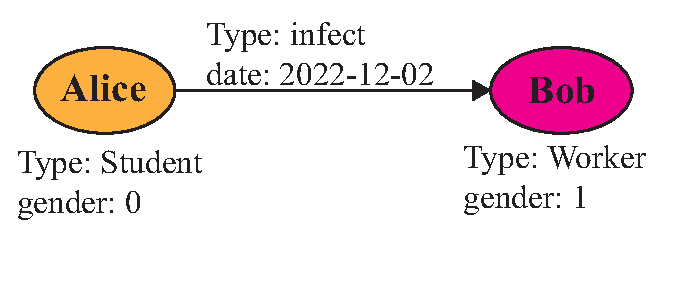
\includegraphics[width=0.45\textwidth]  {figures/propertyG.eps}} 
\bicaption{一个简单的属性图示例}{A simple property graph example}
\label{propertyG}
\end{figure}

\subsection{RDF图}
RDF(Resource Description Framework,资源描述框架)主要用于表示万维网(World Wide Web)上资源之间的关联关系,它是随着语义网的发展而被提出并逐渐流行起来的。
语义网的目标是赋予万维网上的资源以计算机可以理解的元数据,RDF的作用就是使用一种基于图的数据模型来表示万维网上不同资源之间的关系。
RDF数据集的基本组成单元是三元组;每个三元组都由主语(subject)、谓词(predicate)和宾语(object)三个部分组成,可以用 <s, p, o> 的形式来表示。
三元组中的 s 和 o 对应图中的顶点,每个三元组对应图中的一条从顶点 s 指向顶点 o 的一条类型为 p 的有向边。
此外,RDF标准还包含一些预定义的规则,例如使用谓词\texttt{rdf:type}来描述资源的类型。
图\ref{rdf}是一个简单的RDF数据集,它由7个三元组组成,其中4个三元组用于描述资源的类型,3个三元组用于描述资源间的关系。
它对应的RDF图包含四个顶点和三条边。

\begin{figure}[htb]
\centering
\begin{minipage}{.32\linewidth}
\centering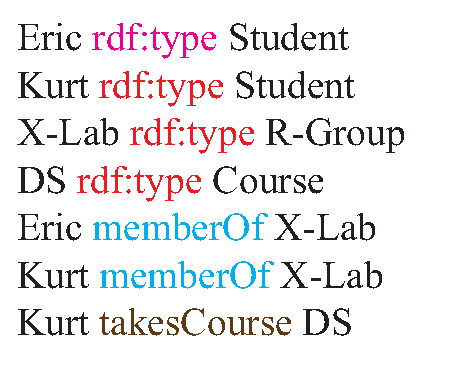
\includegraphics[scale=0.5]{figures/rdfdata.eps}
\end{minipage}
\begin{minipage}{.53\linewidth}
\centering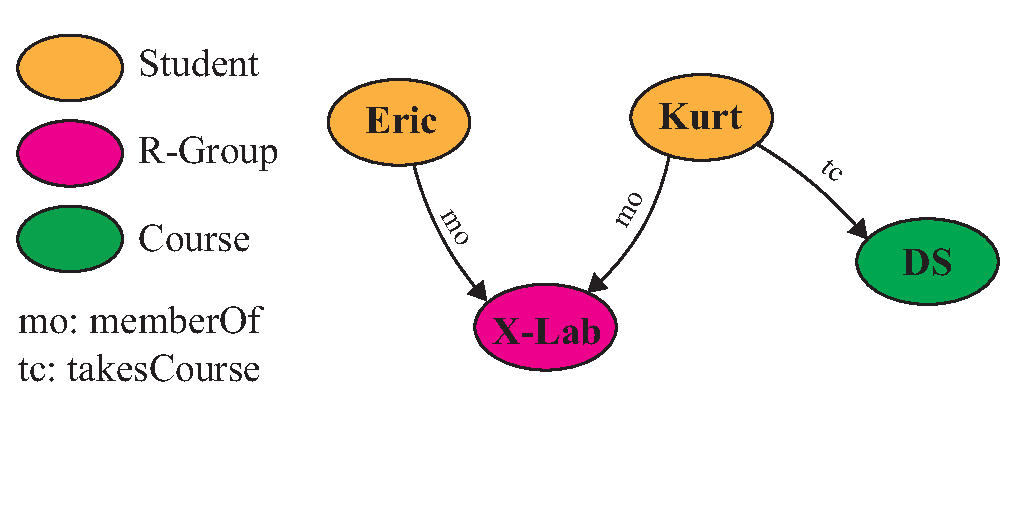
\includegraphics[scale=0.5]{figures/rdf.eps}
\end{minipage}
%\hspace*{2mm}
\begin{minipage}{1\linewidth}
\bicaption{RDF图示例}{An example of RDF graph}
\label{rdf}
\end{minipage}
\end{figure}

SPARQL\upcite{sparql}是RDF图的标准查询语言,一条 SPARQL 查询语句通过指定一个图模式来从 RDF 图中寻找与之匹配的子图。
SPARQL查询语句最常用的形式为:
\begin{eqnarray}
    \mathtt{SELECT \ RD \ WHERE \ GP}
\end{eqnarray}

其中GP是一组“主语-谓词-宾语”三元模式(TP),RD(Result Description,结果描述)是一组变量。
三元模式的每个元素都既可以是变量,也可以是常量。
除了三元模式外,GP中还可以包含过滤器,过滤器的作用是对变量的取值按照一定条件进行过滤。
RD是GP中变量的非空子集,告诉SPARQL执行引擎应该输出哪些变量的取值。
给定一个RDF图$G$和一个SPARQL查询语句$Q$,SPARQL执行引擎会在$G$上搜索与$Q$的GP匹配的子图,找到RD中所有变量的可取值。

图\ref{sparql}(a)给出了一条示例SPARQL查询语句,它想要找到满足如下条件的资源Y:Y的类型是课程且有X-Lab的成员选修该课程。
在图\ref{rdf}中寻找与图\ref{sparql}(b)所示的查询图相匹配的子图,最终可以得到如图\ref{sparql}(c)所示的查询结果。
由于RD只包含一个变量Y,所以查询结果仅有一列,变量Y仅可以取值DS,所以查询结果只有一行。

\begin{figure}[htb] 
\center{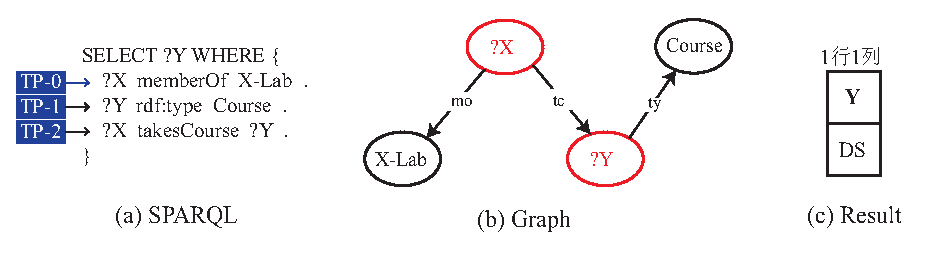
\includegraphics[width=0.9\textwidth]  {figures/sparql.eps}} 
\bicaption{示例RDF图上的一条SPARQL查询语句}{A SPARQL query statement on the RDF graph example}
\label{sparql}
\end{figure}

\subsection{超图}
超图(hypergraph)是在图的基础上泛化的一种数据结构。
普通图中的边只能与两个顶点相连接,而超图中的边能够连接任意数量的顶点。普通图只能描述二元关系,
超图能够描述多元关系。超图同样可以使用$G=(V,E)$来表示,其中$V$是超图中顶点的集合,$E$是超边的集合。
每条超边都是$V$的一个非空子集,它规定了这个集合中包含的所有顶点之间的关系。
事实上,无向图就是一种特殊的超图,这种超图的每条超边都只连接两个顶点。
类似于属性图,超图中的顶点和超边都可以拥有类型和属性。

超图非常适合用来表示可以抽象成集合的数据,例如,一个微信群聊中通常包含几个到几百个微信用户,我们可以把微信群聊抽象为超
边,把微信用户抽象为顶点,如果一个微信用户是某个群聊的成员,那么它对应的顶点就是该群聊对应超边连接的顶点之一。
图\ref{hyper}所示的超图包含 7 个顶点和 3 条超边,群聊$e_1$包含$u_1$和$u_2$两个微信用户,
群聊$e_2$包含$u_2$、$u_3$、$u_4$和$u_5$四个微信用户,$u_2$是这两个群聊的公共成员。

\begin{figure}[htb] 
\center{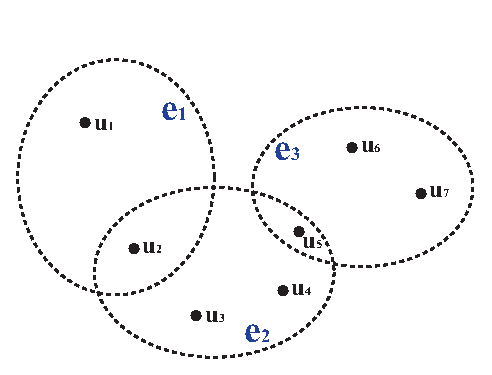
\includegraphics[width=0.4\textwidth]  {figures/hyper.eps}} 
\bicaption{用超图表示的微信群聊关系}{WeChat group relationship represented by hypergraph}
\label{hyper}
\end{figure}

\section{时序图}
属性图、RDF图和超图模型都有各自的时序版本。

在时序属性图中,顶点、边、顶点的各属性和边的各属性都可以有对应的生命周期,这样,顶点和边就可以被添加和删除,顶点和边上的属性在不同的时期也可以有不同的值。
时序属性图的正式定义为:

\begin{definition}[时序属性图]
  时序属性图可以表示为$G=(V,E)$,其中$V$是顶点$v=(vid, \tau_v)$的集合($vid$是其唯一ID,$\tau_v=[t_s, t_e)$是其生命周期时间区间),$E$是边$e=(eid, uid, vid, \tau_e)$的集合($eid$是其唯一ID,$uid, vid\in V$分别是其起点和终点,$\tau_e=[t_s', t_e')$是其生命周期时间区间)。
\end{definition}

时序属性图需要满足一个完整性约束:边的生命周期不能超出它所连接的两个顶点的生命周期。
图\ref{interval}给出了一个满足完整性约束的时序属性图示例,它包含五个顶点和六条边。顶点的生命周期都是$[0,10)$,不同边的生命周期不尽相同,例如顶点$A$和顶点$B$之间有两条边,生命周期为$[0,1)$的边的属性值为$3$,生命周期为$[1,4)$的边的属性值为$7$。

\begin{figure}[htb] 
\center{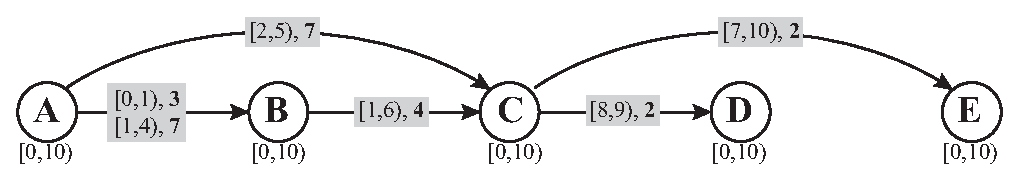
\includegraphics[width=0.9\textwidth]  {figures/interval.eps}} 
\bicaption{时序属性图示例}{An example of temporal property graph}
\label{interval}
\end{figure}

时序RDF图并没有统一的标准定义,结合之前工作对时序RDF图的定义,本文把时序RDF图定义为:

\begin{definition}[时序RDF图]
  时序三元组是带有整数有效时间标签的三元组,可以表示为$(s,p,o):[t]$。时序RDF图就是时序三元组的集合。
  我们使用$(s,p,o):[t_1,t_2)$来简记$\{(s,p,o):[t]|t_1\leq t<t_2,t\in Z\}$,它表示三元组$(s,p,o)$在$[t_1,t_2)$这个时间区间上是有效的。
\end{definition}

图\ref{trdf}是一个时序RDF数据集示例,它是图\ref{rdf}中的RDF图的时序版本,由7个时序三元组组成。
它构成的时序RDF图包含三条边,这三条边都有各自的有效时间区间,例如Eric和X-Lab之间的边的有效时间区间是$[1,2)$。

\begin{figure}[htb]
\centering
\begin{minipage}{.35\linewidth}
\centering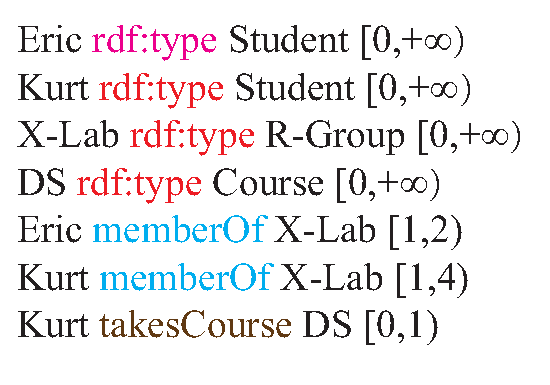
\includegraphics[scale=0.5]{figures/trdfdata.eps}
\end{minipage}
\begin{minipage}{.55\linewidth}
\centering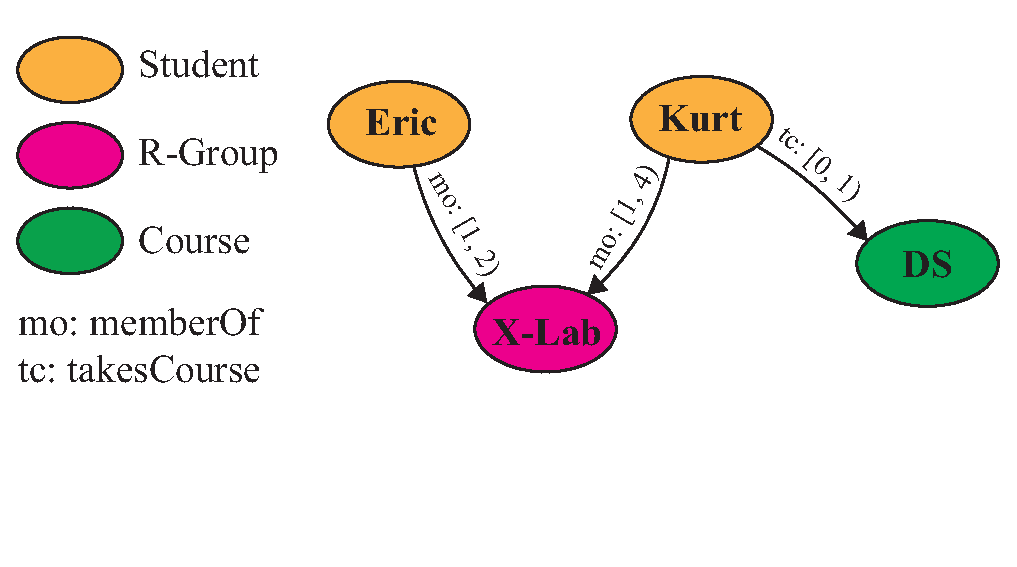
\includegraphics[scale=0.5]{figures/trdf.eps}
\end{minipage}
%\hspace*{2mm}
\begin{minipage}{1\linewidth}
\bicaption{时序RDF图示例}{An example of temporal RDF graph}
\label{trdf}
\end{minipage}
\end{figure}

时序超图同样没有标准的定义,本文把时序超图定义为:

\begin{definition}[时序超图]
  顶点集合$V=\{v_1,...,v_{|V|}\}$上的时序超图$G=(V,E)$是一个时序超边的集合$E=\{e_1,...,e_{|E|}\}$,
  每条时序超边$e=\widetilde{e}:[t]\in E $都是一个带有整数有效时间标签$t$的顶点集合$V$的非空子集。
  我们使用$\widetilde{e}:[t_1,t_2)$来简记$\{\widetilde{e}:[t]|t_1\leq t<t_2,t\in Z\}$,
  它表示时序超边$\widetilde{e}$在$[t_1,t_2)$这个时间区间上是有效的。
\end{definition}

在时序超图中,时序超边和顶点都是可以有类型的。图\ref{thyper}是一个时序超图示例,它是图\ref{hyper}中超图的时序版本,它包含三条时序超边,都有各自的有效时间区间,例如$e_1$表示的微信群聊状态只在时间区间$[1,3)$内是成立的。

\begin{figure}[htb] 
\center{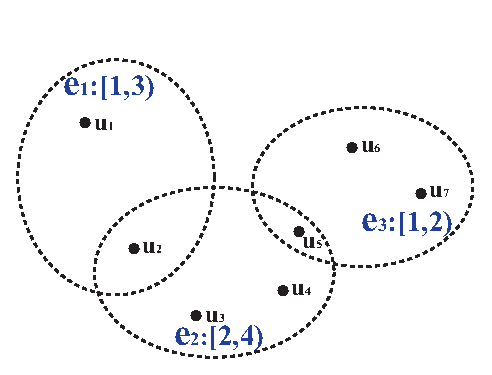
\includegraphics[width=0.4\textwidth]  {figures/thyper.eps}} 
\bicaption{用时序超图表示的微信群聊关系}{WeChat group relationship represented by temporal hypergraph}
\label{thyper}
\end{figure}

\section{Wukong介绍}
\sys 的时序图查询模块是在Wukong的基础上实现的。
Wukong是一个先进的分布式RDF图查询系统,它基于RDMA这一新型硬件特性,通过一系列存储结构和查询引擎上的优化技术,实现了SPARQL查询的低时延、高并发执行。

RDMA(Remote Direct Memory Access,远端内存直接访问)是一种高性能的跨机器内存访问技术,能够以很低的延迟直接访问远端机器的内存。
RDMA操作主要分为两类:单边(one-sided)操作和双边(two-sided)操作。
单边操作可以不经过远端机器的CPU直接读、写其内存,也不需要操作系统内核的参与。
双边操作类似于传统消息传递模式,即分别使用SEND和RECV两个接口进行消息的发送和接收。
虽然双边操作需要服务端CPU的参与,但由于双边操作中的网络协议栈完全由支持RDMA的网卡硬件实现,因此相较于传统基于TCP/IP协议的消息传递,RDMA双边操作仍然能有超过一个数量级的性能提升。

接下来,本文将从存储结构和查询引擎两个方面对Wukong作简要介绍。

\begin{figure}[htb]
\center{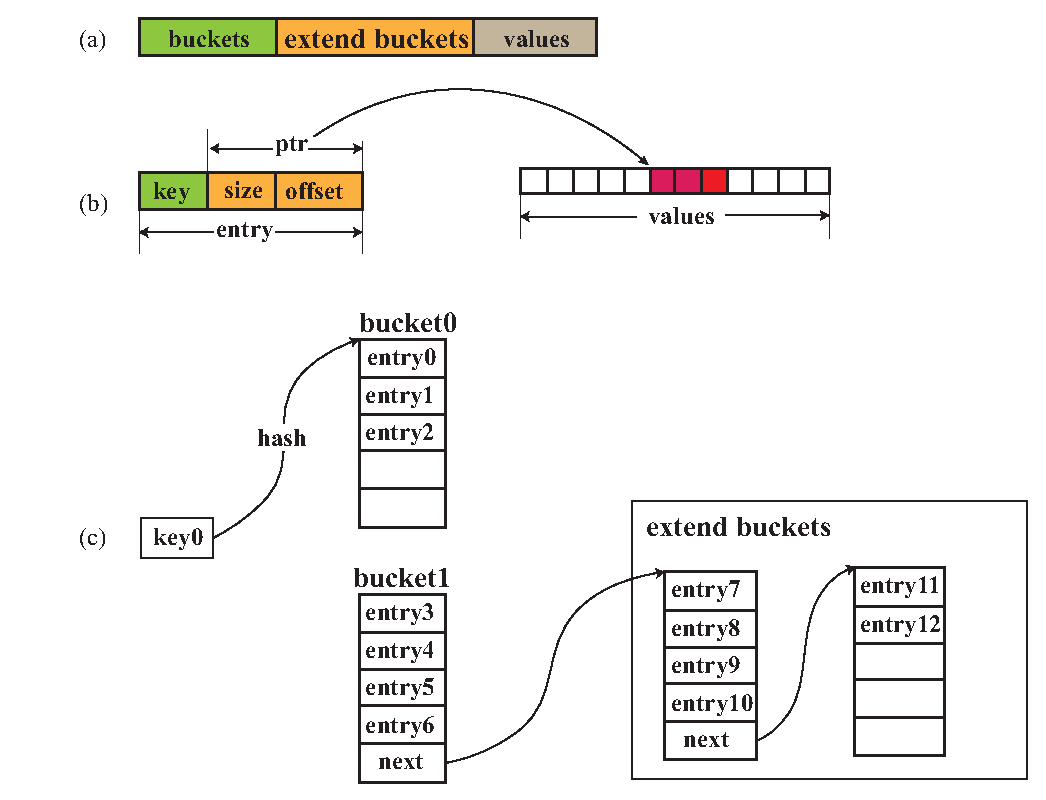
\includegraphics[width=0.8\textwidth]  {figures/kvstore.eps}} 
\bicaption{Wukong的分布式键值存储结构}{Wukong's distributed key-value store structure}
\label{kvstore}
\end{figure}

\subsection{存储结构}
\label{chap:kvstore}
为了充分发挥RDMA在远端内存访问上的性能优势,Wukong使用多机内存实现RDF图数据集的可扩展存储,使用单边RDMA操作访问远端机器的内存。Wukong的基本存储结构是一个如图\ref{kvstore}的分布式键值存储结构。
每台机器上的键值存储由图\ref{kvstore}(a)所示的三块连续的内存区域组成,其中buckets和extend buckets是键和它对应值的位置信息的存储区域,values是值的存储区域。
一个键和它对应值的位置信息组成一个图\ref{kvstore}(b)中的entry,其中key是键本身,size和offset分别是该键对应值的长度(值是一个列表)和位置(相对于values区域起始位置的偏移量)。
如图\ref{kvstore}(c)所示,buckets和extend buckets区域由一系列桶(bucket)组成,每个桶都有$N$个槽(slot),最多可以容纳$N-1$个entry。
给定一个key,系统会使用一个哈希函数计算它对应的entry应该被放在buckets区域中的哪个桶里,当桶满(同一哈希值的key的数量超过$N-1$)时,系统会从extend buckets里分配新桶来继续存放剩下的条目,满桶的最后一个槽会被用来存放指向新桶的指针,形成一个类似于链表的结构。

\begin{algorithm}[htb]
\caption{根据给定键读取对应值}
\label{algo:readkv}
\SetKwInOut{Input}{输入}
\SetKwInOut{Output}{输出}
\SetKw{KwTo}{in}
\SetKwFunction{Range}{range}
\SetKwFor{For}{for}{\string:}{}
\SetKwIF{If}{ElseIf}{Else}{if}{:}{elif}{else:}{}
\SetKwFor{While}{while}{:}{}
\newcommand{\forcond}{$i$ \KwTo\Range{$N$}}
\Input{key}
\Output{值数组}
server\_id $\leftarrow$ hash\_server(key)\;
bucket\_id $\leftarrow$ hash\_bucket(key)\;
slot $\leftarrow$ NULL\;
\While{true}{
    rdma\_offset $\leftarrow$ bucket\_id $\times N \times$ sizeof(slot)\;
    rdma\_size $\leftarrow$ $N \times$ sizeof(slot)\;
    slots $\leftarrow$ RdmaRead(server\_id, rdma\_offset, rdma\_size)\;
    \For{\forcond}{
        \If{$i<N$}{
            \If{slots[$i$].key = key}{
                slot $\leftarrow$ slots[$i$]\;
                goto $read$\;
            }
        }
        \Else{
            \If{IsEmpty(slots[$i$])}{
                goto $read$\;
            }
            bucket\_id $\leftarrow$ slots[$i$].bid\;
        }
    }
}
$read:$
\BlankLine
    \If{slot = NULL}{
        \Return $[]$\;
    }
    \Else{
        \Return RdmaRead(server\_id, values\_base + slot.offset $\times$ sizeof(value), slot.size $\times$ sizeof(value))\;
    }
\end{algorithm}

算法\ref{algo:readkv}给出了根据给定key读取对应值的伪代码。系统首先会通过两个哈希函数计算该key会被存储在哪台机器的哪个桶里(1-2行),然后通过RDMA的单边读操作从相应机器把整个桶都读取过来(5-7行),遍历桶的前$N-1$个槽,对比每个entry的key是否和给定key匹配,如果找不到一致的entry,则通过第N个槽提供的指针继续查找extend buckets区域里的槽(16行),直到寻找到匹配的entry或扫完最后一个桶。
如果搜索到匹配的entry,直接通过RDMA的单边读操作从相应机器的values区域的正确位置读取值即可(21行)。

\subsection{查询引擎}
\label{chap:engine}
Wukong的查询执行引擎使用图探索和全历史剪枝算法执行SPARQL语句。
以图\ref{sparql}中的查询语句为例,图\ref{engine}展示了该语句的执行过程。
查询引擎依次处理语句中的三元模式(\ding{182}),对于每个三元模式,查询引擎会通过构造合适的key从系统的分布式键值存储中查找与该三元模式匹配的子图,这一过程称为图探索。
每个子图都对应着查询语句中变量的一组取值,执行完每个三元模式后探索到的所有子图对应的变量的取值构成中间结果表。
所有三元模式都执行完毕后,中间结果表中RD对应的列就作为最终的查询结果返回给用户。
例如,变量$?X$和$?Y$的所有可取值在TP-1执行完毕后已经被找到,三元模式TP-2的目的是从中筛选出存在takesCourse关系的变量$?X$和$?Y$的取值。
在执行三元模式TP-2时,查询引擎会将中间结果表第一列中的每个值(变量$?X$的取值,\ding{183})分别与三元模式中的谓词常量takesCourse构成key(\ding{184}),从分布式键值存储中读取对应的值(\ding{185}),当且仅当第二列中的值出现在\ding{185}中,该行才会被保留在中间结果表中。
这种通过之前步骤的历史信息精确地修剪掉无用中间结果的的方法就是全历史剪枝。

\begin{figure}[htb]
\center{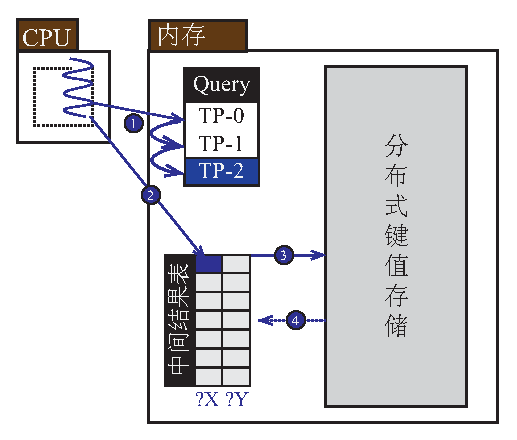
\includegraphics[width=0.5\textwidth]  {figures/engine.eps}} 
\bicaption{SPARQL查询执行过程}{SPARQL query execution process}
\label{engine}
\end{figure}

\section{图分析系统的图存储结构}
CSR (Compressed Sparse Row)是静态图分析系统广泛使用的图存储结构,它是稀疏矩阵的紧凑化表示,图\ref{csr}(a)是一个简单的图拓扑,图\ref{csr}(b)是它的CSR表示,CSR由一个顶点数组和一个边数组组成,其中边数组按照边的起点ID的顺序来存储每条边的终点ID,顶点数组通过顶点的ID来索引,它存储各个顶点的出边在边数组中起始位置的偏移量。在在线图分析场景中,图拓扑会不断更新,而CSR是一种紧凑的结构,在CSR上做图拓扑更新的效率很低,例如,如果在\ref{csr}(a)的图结构中添加一条从顶点0指向顶点3的边,它的CSR表示就需要对顶点数组和边数组做大量更新(如图\ref{csr}(c))

\begin{figure}[!htb]
\center{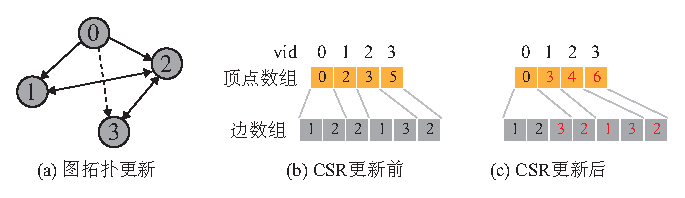
\includegraphics[width=0.8\textwidth]  {figures/csr-update.eps}} 
\bicaption{图拓扑的CSR表示}{CSR representation of graph topology}
\label{csr}
\end{figure}

在线图分析系统(例如RisGraph\cite{risgraph}、GraphOne\cite{graphone}和LiveGraph)和动态图存储(例如CSR++\cite{csrpp}和Sortledton\cite{sortledton})通常使用邻接列表作为图拓扑存储的基本数据结构。
如图\ref{adja}(a),使用邻接列表表示图拓扑时,每个顶点的所有出边的终点ID都会被存放在一个单独的邻接列表中,邻接列表指针数组存放指向每个邻接列表的指针。如图\ref{adja}(b),在添加一条从顶点0指向顶点3的边时,只需要往顶点0的邻接列表中添加一个元素3即可。逐顶点的邻边扫描(以下简称扫边)是图分析中最常用的操作。图拓扑的邻接列表表示虽然具有更高的图更新效率,但它的结构较为松散,在扫边过程中的数据局部性较差,扫边性能远不及图拓扑的CSR表示。
\begin{figure}[!htb]
\center{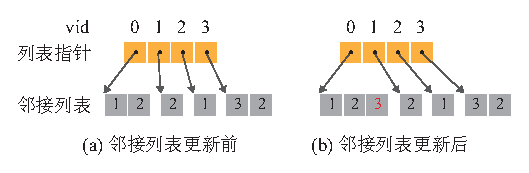
\includegraphics[width=0.6\textwidth]  {figures/adja.eps}} 
\bicaption{图拓扑的邻接列表表示}{Adjacency list representation of graph topology}
\label{adja}
\end{figure}

\section{本章小结}
本章介绍了与本工作相关的背景知识。
属性图、RDF 图和超图是定义图结构的三大范式。
属性图是最为常用的建模图状结构数据的模型;
RDF的作用是使用一种基于图的数据模型来表示万维网上不同资源之间的关系,SPARQL是RDF图的标准查询语言;超图是在图的基础上泛化的一种数据结构,超图中的边能够连接任意数量的顶点。随着时间而变化的图叫做时序图,属性图、RDF图和超图都有各自的时序版本。
本文给出了时序属性图的正式定义,然后结合之前工作给出了时序RDF图和时序超图的定义。
\sys 的时序图查询模块是在Wukong的基础上实现的,本章从存储结构和查询引擎两个方面对Wukong进行了简要介绍。
CSR和邻接列表是图分析系统常用的两种图存储结构,它们分别适用于离线和在线图分析系统。
\chapter{\sys 的总体架构}
\sys 是一个同时支持时序图查询和第一类时序图分析的图处理系统,它由时序图查询和时序图分析两大模块组成。传统的图处理系统通常是基于单一图模型实现的,例如Neo4j是一个基于属性图模型的图数据库,而\sys 将时序属性图、时序RDF图和时序超图三种时序图模型集成到同一系统中。具体来说,\sys 的时序图查询模块同时支持时序RDF图和时序超图两种时序图模型,而时序图分析模块则是基于时序属性图模型实现的。本章将首先介绍系统的总体架构,然后详述系统接口层的实现。

\section{架构概述}
\label{sec:arch}
\sys 的系统架构如图\ref{arch},系统运行在一个由RDMA网络相互连接的集群环境中。
在一个机器数量为$N+2$的集群中,每台机器运行一个服务节点。其中,一个字符串服务器节点用于处理字符串和整型ID之间的转换,一个节点负责处理图的事务化更新和执行系统管理员发起的时序图分析任务(下称分析节点),其余$N$个节点负责处理来自用户的时序RDF图查询请求和时序超图查询请求(下称查询节点)。

\begin{figure}[htb]
\center{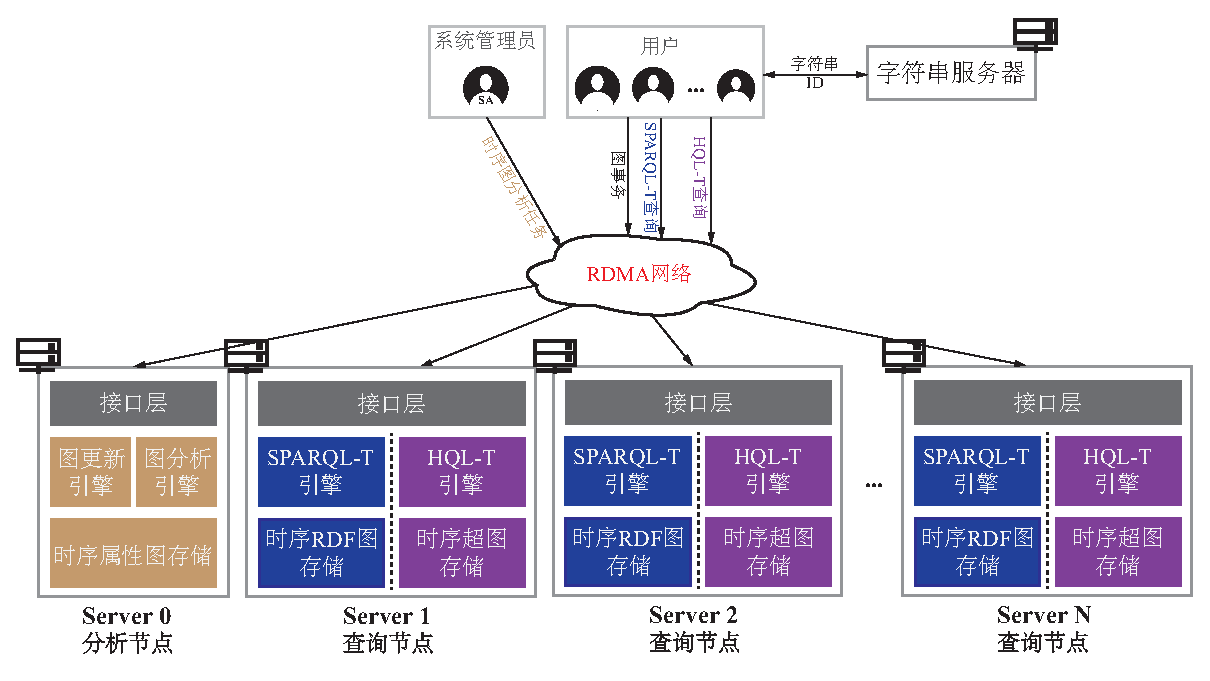
\includegraphics[width=0.87\textwidth]  {figures/arch.eps}} 
\bicaption{\sys 的系统架构}{The architecture of \sys}
\label{arch}
\end{figure}

由于时序RDF图和时序超图都没有标准的查询语言,所以本文设计了系统支持的时序RDF图查询语言和时序超图查询语言,分别命名为SPARQL-T和HQL-T。
在时序RDF图数据集中,时序三元组的主语、谓词和宾语都是字符串,时序超图数据集中的超边名和顶点名也都是字符串。
\sys 在存储时序数据集时,并不直接存储字符串,而是将字符串转化成整型ID进行存储,字符串服务器节点存储了字符串和整型ID之间的映射并负责转换,这一方面减少了系统的内存使用量,另一方面将字符串匹配转换成整型的匹配,加快了匹配速度。用户在发起SPARQL-T和HQL-T查询请求时,会先和字符串服务器节点通信,将查询语句中的字符串转换成整型ID,然后再把它交给系统执行;用户在收到系统返回的查询执行结果时,同样会和字符串服务器节点通信,将查询结果中的ID转回字符串。

\sys 的时序图查询模块采用了去中心化的分布式架构,它采用边割\cite{edgecut}的方式将时序图数据分区存储到$N$个查询节点的内存中以实现水平扩展(章节\S\ref{sec:rdfstore}和\S\ref{sec:hyperstore})。$N$个查询节点是对等的,都能接收和执行来自用户的时序图查询请求,并可以通过RDMA网络实现跨节点的协作,进而提高查询执行的局部性和并行性,提高查询的执行效率。系统的时序图分析模块是单机的,来自用户的图事务请求和来自系统管理员的时序图分析任务都会被转发到分析节点,分别由分析节点的事务处理线程和时序图分析线程来完成。

分析节点和查询节点存储的图数据是相互独立的,查询节点中的时序RDF图和时序超图存储也是相互独立的,图事务请求和时序图分析任务需要读写的是分析节点中的时序属性图存储,SPARQL-T和HQL-T查询请求查询的分别是时序RDF图存储和时序超图存储中的图数据。
由于分析节点需要同时支持图事务和时序图分析,所以时序属性图存储是可读可写的。查询节点只需要支持对时序图数据的检索,时序图数据被加载完毕之后便不会再被更新,因此时序RDF图存储和时序超图存储都是只读的。

除了字符串服务器节点外,系统中的每个节点都由存储层、引擎层和接口层三层组成。存储层负责图数据的存储,并提供访问和更新接口(仅分析节点的存储层提供更新接口)供引擎层使用;引擎层负责图更新、查询和分析任务的执行,它需要使用存储层提供的接口来读写图数据;接口层负责接收来自于用户或系统管理员的请求,将它们解析为系统的内部表示,然后分配给特定节点的引擎层执行。

\section{接口层}
\label{chap:interface}
如\S\ref{sec:arch}所述,接口层负责请求的接收、解析和分配。
接口层由分析节点和查询节点上的若干代理线程和为每个代理线程准备的专用缓冲区来实现。
每个节点的接口层都是对等的,每个代理线程都可以接收和解析来自用户或系统管理员的请求。
节点上的线程分为代理线程和工作线程两种,代理线程位于接口层;工作线程位于引擎层,负责任务的实际执行。
对于分析节点,工作线程又可以分成图事务处理线程和时序图分析处理线程两类;对于查询节点,工作线程负责执行时序图查询任务。
每个线程都有一个专用的缓冲区,线程按照FIFO的顺序从缓冲区中读取请求或结果,本地节点的线程可以直接写缓冲区,远程节点的线程通过单边RDMA Write操作写缓冲区。
代理线程的缓冲区用于接收工作线程的执行结果,工作线程的缓冲区用于接收代理线程或其他工作线程发来的请求。
每个缓冲区被分为$N+1$块,编号为$0, 1, ..., N$,编号为$i (0\leq i \leq N)$的节点只能写缓冲区的第$i$块,这样可以保证不同节点的线程对缓冲区的写不会相互干扰,不需要锁的参与,从而实现节点内和跨节点的高效线程间通信。

\begin{figure}[htb]
\center{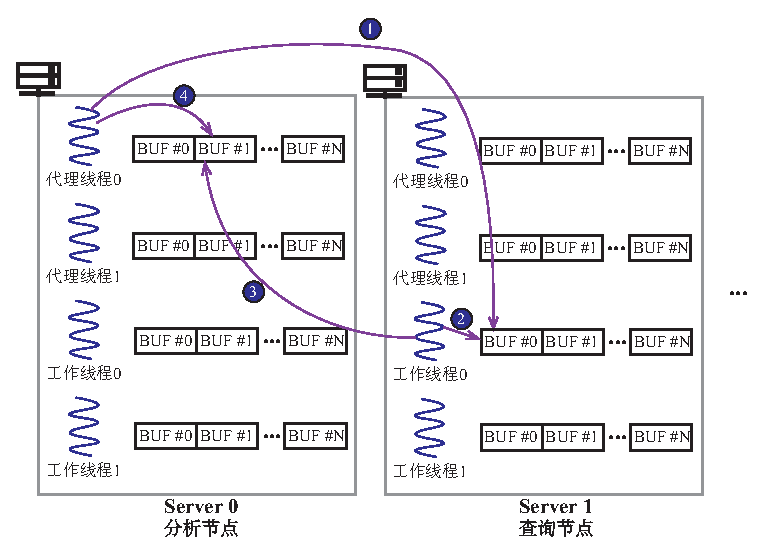
\includegraphics[width=0.7\textwidth]  {figures/interface.eps}} 
\bicaption{线程间的通信流程}{The communication flow between threads}
\label{interface}
\end{figure}

图\ref{interface}演示了线程间的通信流程。
代理线程接收并解析完成请求后,会将请求发送给适当节点的工作线程执行(\ding{182}),方法是使用单边RDMA Write操作写或直接本地写工作线程对应缓冲区中供代理线程所在节点使用的块,然后代理线程会轮询其缓冲区,等待执行结果。
工作线程会轮询其缓冲区,从中读取请求(\ding{183})开始执行。
执行完成后,工作线程会将结果发回代理线程(\ding{184}),方法同样是使用单边RDMA Write操作写或直接本地写代理线程对应缓冲区中供工作线程所在节点使用的块。
此时代理线程就可以读取到请求结果(\ding{185})并返回给用户。

步骤\ding{182}中应该将请求发送给哪个节点的哪个工作线程由以下两个准则决定:
\begin{itemize}
    \item 图事务和时序图分析请求分别会被发送给分析节点的随机图事务工作线程和时序图分析工作线程处理;
    \item 时序图查询请求会被发送给能够使得数据局部性最好的查询节点的随机工作线程执行。虽然RDMA能够高效地实现对远端内存的读取,但它的性能还是落后于对本地内存的读,我们希望查询能够在使得单边RDMA Read操作尽量少、本地内存读尽量多的节点上被处理。
\end{itemize}

\section{本章小结}
本章介绍了\sys 的系统架构。
系统运行在一个由RDMA网络相互连接的集群环境中,集群包含查询节点、分析节点和字符串服务器节点三类节点。
查询节点用于执行来自用户的SPARQL-T和HQL-T查询语句,分析节点用于处理图事务和时序图分析请求,字符串服务器节点用于处理字符串和整型ID之间的转换。
\sys 的时序图查询模块采用了去中心化的分布式架构,而时序图分析模块则是单机的。
每个查询节点和分析节点都由存储层、引擎层和接口层三层组成。存储层负责图数据的存储,引擎层负责图更新、查询和分析任务的执行,接口层负责请求的接收、解析和分配。
本章还对系统的接口层作了详细介绍。接口层由分析节点和查询节点上的若干代理线程和为每个代理线程准备的专用缓冲区来实现,代理线程和工作线程之间可以通过单边RDMA操作实现高效的线程间通信,从而实现高效的请求的分配和执行结果的获取。
\chapter{时序图查询模块的设计与实现}
时序RDF图和时序超图查询系统是受关注相对较少的研究方向,即使已经出现了一些面向时序RDF图的图查询系统,但它们的性能较差,查询响应时间和并发处理能力都难以令人满意,时序超图查询系统的研究更是少有人问津。本章将介绍\sys 的时序图查询模块,它在Wukong的基础上对时序图查询进行了针对性的优化,实现了时序RDF图和时序超图的可扩展存储和高效查询。

\section{时序图查询语言}
RDF的标准查询语言SPARQL并没有与时序相关的语法,所以需要在SPARQL原有语法的基础上进行时序扩展,以支持时序数据的查询。超图并没有其标准的查询语言,时序超图当然也没有,所以我们同样需要设计时序超图的查询语言。

\subsection{时序RDF图查询语言SPARQL-T}
本文设计的时序RDF图查询语言SPARQL-T从两方面对SPARQL的语法进行了扩展:
\begin{itemize}
\item 将GP中的“主语-谓词-宾语”三元模式扩展为“主语-谓词-宾语-有效时间区间的开始时间-有效时间区间的截止时间”五元模式(QP),新加入的两个元素要求是变量,用来获取时序三元组的有效时间数据。为了兼容标准的SPARQL语法,我们规定新加入的两个元素是可选的,但它们要么同时存在,要么同时不存在。
\item GP中的过滤器可以对时间变量的取值按照一定条件进行过滤,例如与变量或常量的大小关系比较等。
\end{itemize}

\begin{figure}[!htb]
\center{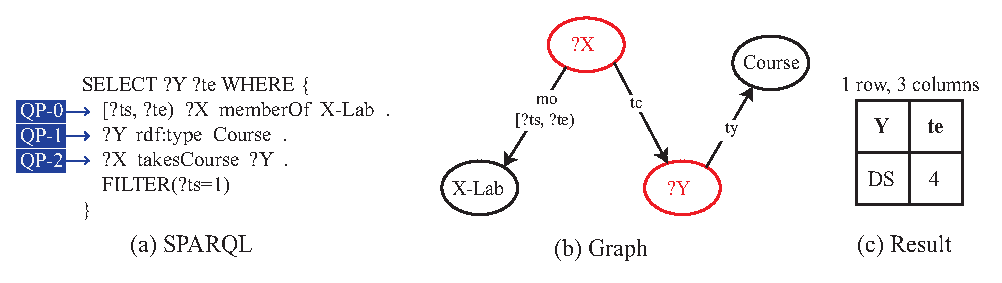
\includegraphics[width=0.9\textwidth]  {figures/tsparql.eps}} 
\bicaption{示例时序RDF图上的一条SPARQL-T查询语句}{A SPARQL-T query statement on the temporal RDF graph example}
\label{tsparql}
\end{figure}

图\ref{tsparql}给出了一条图\ref{trdf}中的时序RDF图上的SPARQL-T语句示例。
QP-0包含两个时间变量\texttt{ts}和\texttt{te},它们应该分别取值为匹配到的时序三元组的有效时间区间的开始时间和截止时间。
GP还包含一个过滤器,它会过滤出变量\texttt{ts}的取值为1的查询结果条目。
GP中的三个模式构成了图\ref{tsparql}(b)所示的查询图,可以在图\ref{trdf}中的时序RDF图上找到一个与之匹配的子图,
过滤后得到的查询结果如图\ref{tsparql}(c)所示,共一行二列。

\subsection{时序超图查询语言HQL-T}
时序超图是一种表示集合关系的数据模型,所以时序超图查询语言应该着重查询\textbf{集合间的关系}(即时序超边间的关系)、\textbf{元素和集合间的关系}(即顶点和时序超边间的关系)以及\textbf{元素间的关系}(即顶点间的关系)。此外,时序超图查询语言也应当支持\textbf{对时序超边的有效时间的查询}以及\textbf{基于有效时间的筛选}。

HQL-T查询语句的基础形式依然是
\begin{equation}
    \mathtt{SELECT \ RD \ WHERE \ GP}
\end{equation}
其中GP由一组基础关系模式(RP)组成,也可以包含过滤器,过滤器和RD的作用与SPARQL-T中的相同。给定一个时序超图$G$和一个HQL-T查询语句$Q$,HQL-T执行引擎会根据GP指定的模式在$G$中搜索与之匹配的子结构,找到RD中所有变量的可取值。RP的基本结构为:
\begin{equation}
    \mathtt{input \ builtin\colon \! type(args) \ output \ interval}
\end{equation}
其中\texttt{input}是输入元素列表,\texttt{builtin}是内置关键字,\texttt{type}指定了该模式的类型,\texttt{args}是该模式的参数,\texttt{output}是输出元素列表。\texttt{interval}是可选的,它是一个由两个变量组成的区间,格式为\texttt{[?var$_1$,?var$_2$)},当它出现在RP中时,HQL-T执行引擎应当将变量\texttt{var$_1$}和\texttt{var$_2$}分别取值为使得此RP成立的时间区间的开始时间和截止时间。
根据\texttt{type}的值,RP可分为以下几类:

\begin{figure}[!htb]
\center{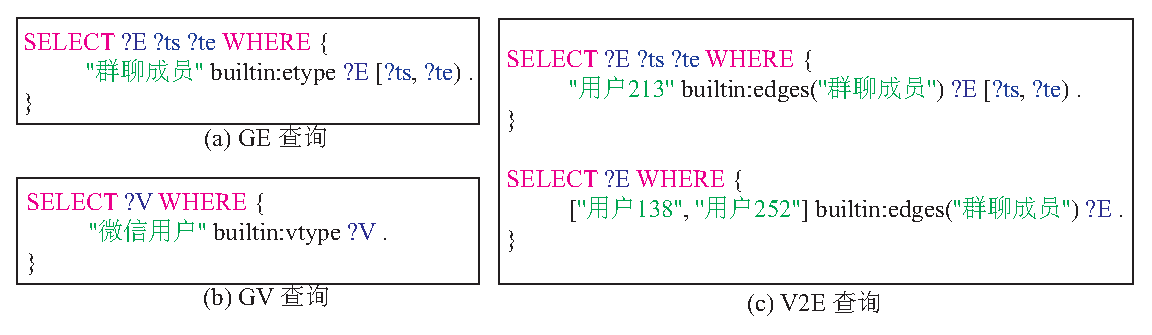
\includegraphics[width=0.9\textwidth]  {figures/hqls1.eps}} 
\bicaption{HQL-T查询语句示例(1)}{HQL-T query statement example (1)}
\label{hql1}
\end{figure}

\begin{itemize}
\item \textbf{GE模式:}该类型RP的\texttt{type}为\texttt{etype},输入元素列表要求只包含一个表示时序超边类型的常量;输出元素列表要求只包含一个变量;没有参数。这类RP的作用是查询所有指定类型的时序超边。如果包含\texttt{interval},那么变量\texttt{var$_1$}和\texttt{var$_2$}会分别取值为查询到的时序超边的有效时间区间的开始时间和截止时间。图\ref{hql1}(a)给出了一条只包含GE模式的HQL-T查询语句示例,该查询是要查找所有类型为“群聊成员”的时序超边。
\item \textbf{GV模式:}该类型RP的\texttt{type}为\texttt{vtype},输入元素列表要求只包含一个表示顶点类型的常量;输出元素列表要求只包含一个变量;没有参数。这类RP的作用是查询所有指定类型的顶点。由于顶点没有时序数据,所以\texttt{interval}不能出现在这类RP中。图\ref{hql1}(b)给出了一条只包含GV模式的HQL-T查询语句示例,该查询是要查找所有类型为“微信用户”的顶点。
\item \textbf{V2E模式:}该类型RP的\texttt{type}为\texttt{edges},输入元素列表可以包含若干表示顶点的常量或变量,输出元素列表要求只包含一个表示时序超边的变量,参数必须是一个表示时序超边类型的常量。这类RP的作用是查找所有指定类型且同时包含各输入顶点的时序超边。如果包含\texttt{interval},那么变量\texttt{var$_1$}和\texttt{var$_2$}会分别取值为查询到的时序超边的有效时间区间的开始时间和截止时间。图\ref{hql1}(c)给出了两条只包含V2E模式的HQL-T查询语句示例,第一个查询是要查找所有类型为“群聊成员”且包含顶点“用户213”的时序超边,第二个查询是要查找所有类型为“群聊成员”且同时包含顶点“用户138”和“用户252”的时序超边。
\end{itemize}

\begin{figure}[!htb]
\center{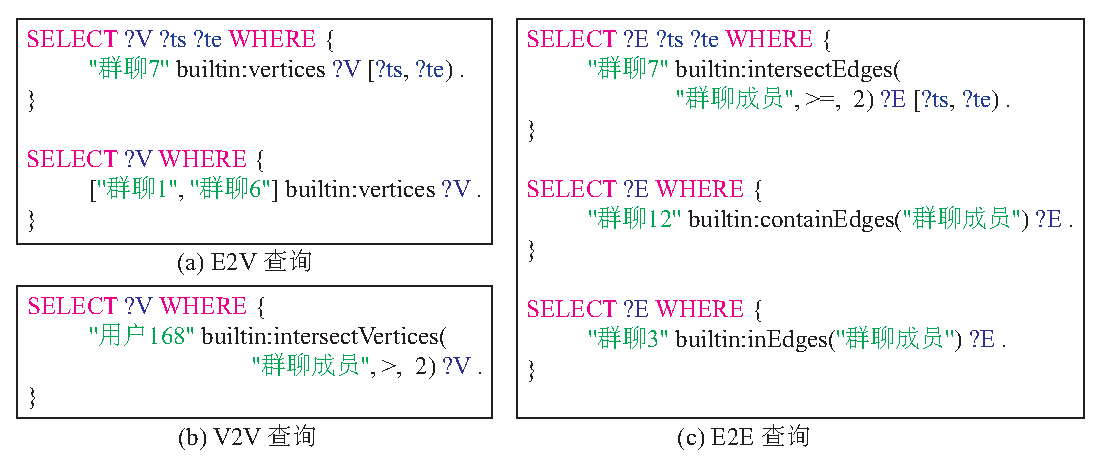
\includegraphics[width=0.9\textwidth]  {figures/hqls2.eps}} 
\bicaption{HQL-T查询语句示例(2)}{HQL-T query statement example (2)}
\label{hql2}
\end{figure}

\begin{itemize}
\item \textbf{E2V模式:}该类型RP的\texttt{type}为\texttt{vertices},输入元素列表可以包含若干表示时序超边的常量或变量,输出元素要求只包含一个表示顶点的变量,没有参数。这类RP的作用是查找各输入时序超边包含的所有公共顶点。如果包含\texttt{interval},那么变量\texttt{var$_1$}和\texttt{var$_2$}会分别取值为能够使得各输入时序超边都有效的最大时间区间的开始时间和截止时间。图\ref{hql2}(a)给出了两条只包含E2V模式的HQL-T查询语句示例,第一个查询是要查找时序超边“群聊7”的有效时间区间和包含的所有顶点,第二个查询是要查找时序超边“群聊1”和“群聊6”包含的公共顶点。
\item \textbf{V2V模式:}该类型RP的\texttt{type}为\texttt{intersectVertices},输入元素列表可以包含若干表示顶点的常量或变量,输出元素要求只包含一个表示顶点的变量。要求有三个参数,第一个参数是时序超边的类型,第二个参数是比较运算符,可以是$>$、$<$、$=$、$!=$、$>=$和$<=$其中之一,该参数可以省略,省略时默认是$>=$,第三个参数是一个整数。这类RP的作用是查找同时与各输入顶点出现在相同时序超边的顶点,且时序超边的类型和数量要满足参数的要求。这类RP不能包含\texttt{interval}。图\ref{hql2}(b)给出了一条只包含V2V模式的HQL-T查询语句示例,该查询是要查找与顶点“用户168”同时加入超过2个共同群聊的顶点。
\item \textbf{E2E模式:}该类型RP的\texttt{type}为\texttt{intersectEdges}、\texttt{containEdges}或\texttt{inEdges},输入元素列表可以包含若干表示时序超边的常量或变量,输出元素要求只包含一个表示时序超边的变量。当\texttt{type}为\texttt{intersectEdges}时,要求有三个参数,第一个参数是时序超边的类型,第二个参数是比较运算符,可以是$>$、$<$、$=$、$!=$、$>=$和$<=$其中之一,该参数可以省略,省略时默认是$>=$,第三个参数是一个整数,这类RP的作用是查找与各输入时序超边的交集的基数满足参数要求的时序超边;当\texttt{type}为\texttt{containEdges}或\texttt{inEdges}时,参数必须是一个表示时序超边类型的常量,这类RP的作用是查找指定类型且是各输入时序超边子集(当\texttt{type}为\texttt{containEdges}时)或超集(当\texttt{type}为\texttt{inEdges}时)的时序超边。如果包含\texttt{interval},那么变量\texttt{var$_1$}和\texttt{var$_2$}会分别
取值为能够使得各输入、输出时序超边同时有效的最大时间区间的开始时间和截止时间。图\ref{hql2}(c)给出了三个只包含E2E模式的HQL-T查询语句示例,第一个查询是要查找与时序超边“群聊7”拥有不少于2个公共顶点的类型为“群聊成员”的时序超边,第二个查询是要查找所有顶点都在时序超边“群聊12”中且类型为“群聊成员”的时序超边,第三个查询是要查找包含时序超边“群聊3”的所有顶点且类型为“群聊成员”的时序超边。
\end{itemize}

以上六类RP的组合可以实现很强的查询语义,基本可以满足对时序超图的查询需求。对于包含多RP的HQL-T查询语句,查询引擎需要按序逐条执行各RP。图\ref{hql}是一条包含两个RP的查询语句,在执行该语句时,需要先找到所有类型为“群聊成员”的时序超边,然后将找到的所有时序超边依次作为输入元素,查找其包含的所有顶点,最后过滤出符合条件的查询结果。

\begin{figure}[!htb]
\center{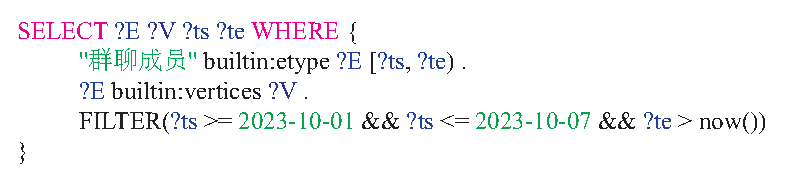
\includegraphics[width=0.8\textwidth]  {figures/hql.eps}}
\bicaption{普通HQL-T查询语句示例}{Common HQL-T query statement example}
\label{hql}
\end{figure}
\section{时序RDF图存储结构和查询引擎}
时序RDF图的存储主要是基于\S\ref{chap:kvstore}中介绍的分布式键值存储实现的,在此基础上,它还使用分布式排序数组结构加速时间条件查询。时序RDF图查询引擎使用存储层提供的接口、按照用户指定的查询计划执行SPARQL-T查询语句中GP的各模式。本节将详细介绍时序RDF图的存储结构和查询引擎。
\subsection{存储结构}
\label{sec:rdfstore}
如\S\ref{sec:arch}所述,\sys 并不直接存储时序RDF图数据集中的字符串,而是将其转化成整型ID进行存储,并使用字符串服务器管理字符串和整型ID之间的对应关系。时序RDF图数据集中的字符串分为两类:
\begin{enumerate}
\item 时序三元组中表示谓词的字符串及表示类型名的字符串,例如时序三元组\texttt{Eric memberOf X-Lab [1,2)}中的\texttt{memberOf}和时序三元组\texttt{Eric rdf:type Student [0,+$\infty$)}中的\texttt{rdf:type}、\texttt{Student}。
这类字符串对应的ID范围为$[1,2^{17})$,特别地,\texttt{rdf:type}对应的ID为1。
本文将表示谓词的字符串对应的ID称为\texttt{pid},将表示类型名的字符串对应的ID称为\texttt{tid}。
\item 时序三元组中表示主语和宾语的字符串(表示类型名的字符串除外),例如时序三元组\texttt{Eric memberOf X-Lab [1,2)}中的\texttt{Eric}和\texttt{X-Lab}。这类字符串对应的ID范围为$[2^{17},2^{46})$。本文将这类字符串对应的ID称为\texttt{vid}。
\end{enumerate}

系统默认使用32位UINT表示各种ID,对于规模比较庞大的数据集,可以在系统编译时指定使用64位UINT。

时序RDF图存储内存布局如图\ref{trdfstore},分为键值存储区和时序三元组存储区两部分。
时序三元组存储区本质上是内存数组,它分为两部分,在“时序三元组存储1”中,时序三元组按照有效时间区间的开始时间升序排布;在“时序三元组存储2”中,时序三元组按照有效时间区间的截止时间升序排布。
键值存储区中的键值对分为直接索引和间接索引两类,在直接索引中,值是实际数据;在间接索引中,值由指向“时序三元组存储1”中时序三元组的指针组成。

\begin{figure}[!htb]
\center{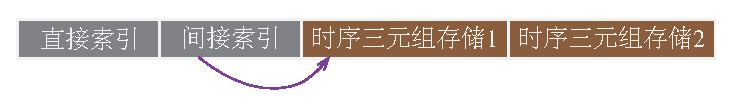
\includegraphics[width=0.6\textwidth]  {figures/trdfstore.eps}}
\bicaption{时序RDF图存储内存布局}{Temporal RDF graph storage memory layout}
\label{trdfstore}
\end{figure}

在键值存储区中,各种键值对及其类型如表\ref{tab:trdf}所示。键的数据类型是64位UINT,由三部分组成,第一部分使用其高46位,第二部分使用其中间17位,第三部分使用其最低位。第三部分只能是OUT(1,表示出方向)和IN(0,表示入方向)其中之一。值的基本数据类型与ID的数据类型相同,可以是32或64位UINT,这取决于系统编译时的配置。
\begin{table}[!hpt]
  \bicaption{时序RDF图存储使用的键值对}{Key-value pairs used in temporal RDF graph storage}
  \label{tab:trdf}
  \centering
  \begin{tabular}{p{1cm}p{3cm}p{8cm}p{2cm}} \toprule
    序号 & 键 & 值 & 类型 \\ \midrule
    1\centering & \texttt{[0|0|OUT]} & 所有\texttt{pid} & \multirow{8}{*}{直接索引} \\
    2\centering & \texttt{[0|1|OUT]} & 所有\texttt{tid} & \\
    3\centering & \texttt{[0|1|IN]} & 所有\texttt{vid} & \\
    4\centering & \texttt{[0|tid|IN]} & 所有类型为\texttt{tid}的\texttt{vid} & \\
    5\centering & \texttt{[0|pid|OUT]} & 谓词为\texttt{pid}的所有时序三元组中所有表示宾语的\texttt{vid} & \\
    6\centering & \texttt{[0|pid|IN]} & 谓词为\texttt{pid}的所有时序三元组中所有表示主语的\texttt{vid} & \\
    7\centering & \texttt{[vid|0|OUT]} & 主语为\texttt{vid}的所有时序三元组中的所有\texttt{pid} & \\
    8\centering & \texttt{[vid|0|IN]} & 宾语为\texttt{vid}的所有时序三元组中的所有\texttt{pid} & \\ 
    \hline
    9\centering & \texttt{[vid|1|OUT]} & 描述\texttt{vid}类型的时序三元组 & \multirow{3}{*}{间接索引} \\ 
    10\centering & \texttt{[vid|pid|OUT]} & 主语为\texttt{vid}、谓词为\texttt{pid}的所有时序三元组 & \\ 
    11\centering & \texttt{[vid|pid|IN]} & 宾语为\texttt{vid}、谓词为\texttt{pid}的所有时序三元组 & \\ 
    \bottomrule
  \end{tabular}
\end{table}

图\ref{trsdemo}给出了系统会为图\ref{trdf}中的数据集生成的一部分键值对。为了便于理解,图中使用字符串表示主语、谓词和宾语,系统实际使用的是这些字符串对应的ID。
在间接索引中,值是一个由时序三元组在“时序三元组存储1”中的偏移量组成的列表,例如,时序三元组\texttt{Kurt memberOf X-Lab [1,4)}在“时序三元组存储1”中的偏移量为5,那么间接索引就使用5来表示该时序三元组。

\begin{figure}[!htb]
\center{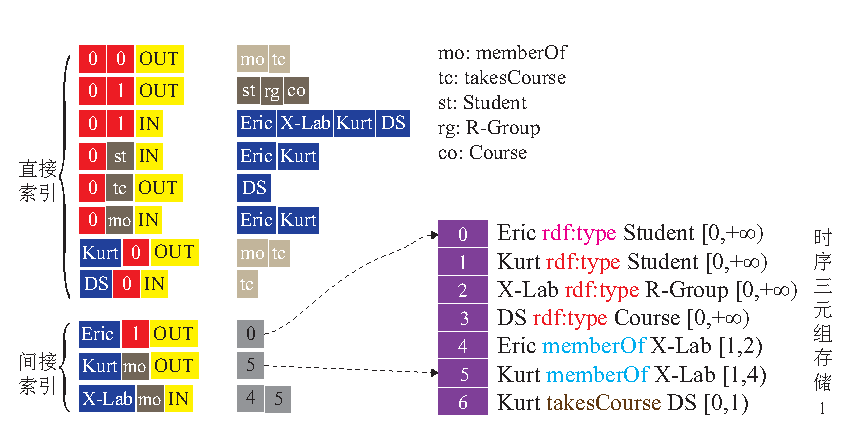
\includegraphics[width=0.75\textwidth]  {figures/trsdemo.eps}}
\bicaption{时序RDF图存储使用的键值对示例}{Example of key-value pairs used in temporal RDF graph storage}
\label{trsdemo}
\end{figure}

为了实现RDF数据集的分布式可扩展存储,系统使用如下规则将键值对和时序三元组划分到各查询节点中存储:
\begin{enumerate}
    \item 每个查询节点负责一部分\texttt{vid}的管理,\texttt{vid}会被分配到的查询节点(查询节点从0开始编号)为:
    \begin{equation}
        \mathtt{vid \ \% \ num\_qnodes}
    \end{equation}
    其中\texttt{num\_qnodes}是查询节点数。
    \item 对于键值对1-6,将值按照1中的规则划分到各查询节点存储,同一键会出现在每个查询节点的键值存储中;对于键值对7-11,将键依据其第一部分按照1中的规则划分到不同查询节点存储,每个键只会出现在一个查询节点的键值存储中。
    \item 将所有时序三元组分别按有效时间区间的开始时间和截止时间排序后,分别按块划分到各查询节点的“时序三元组存储1”和“时序三元组存储2”中存储,偏移量为\texttt{off}的时序三元组会被分配到的查询节点(从0开始编号)为:
    \begin{equation}
        \mathtt{off \ / \ \lceil num\_ttriples \ / \ num\_qnodes \rceil}
    \end{equation}
    其中\texttt{num\_ttriples}是时序三元组总数。
\end{enumerate}

分布式键值存储结构可以实现高效的拓扑查询,两个“时序三元组存储”可以实现高效的时间条件查询。对于以时序三元组有效时间区间开始时间为条件的查询,可以在“时序三元组存储1”上通过二分法快速找到目标时序三元组,同理可以使用“时序三元组存储2”快速处理以时序三元组有效时间区间截止时间为条件的查询。直接索引和间接索引相结合的键值存储结构可以在实现高效的拓扑查询和时间条件查询的同时,减少时序数据存储占用的空间。

表\ref{tab:storeif}列出了存储层向上提供的接口,接口\ding{182}只涉及对本节点上键值存储结构的读,接口\ding{183}可能涉及对各节点的键值存储结构和“时序三元组存储1”的读,接口\ding{184}和\ding{185}可以分别筛选出本节点的“时序三元组存储1”和“时序三元组存储2”中符合时间条件的时序三元组。
\begin{table}[!hpt]
  \bicaption{时序RDF图存储提供的接口}{Interfaces provided by temporal RDF graph storage}
  \label{tab:storeif}
  \centering
  \begin{tabular}{p{1cm}p{8cm}p{5.5cm}} \toprule
    序号 & 接口 & 作用 \\ \midrule
    \ding{182}\centering & \texttt{list<value\_t> get\_values(key)} & 获取本节点上键\texttt{key}对应的值列表,适用于键值对1-6 \\
    \ding{183}\centering & \texttt{list<triple\_t> get\_ttriples(key)} & 获取键\texttt{key}对应的时序三元组列表,适用于键值对7-11 \\
    \hline
    \ding{184}\centering & \texttt{list<triple\_t> get\_ttriples\_ts(start, end)} & 从本节点的“时序三元组存储1”中获取所有有效时间区间开始时间范围为\texttt{[start,end]}的时序三元组 \\
    \ding{185}\centering & \texttt{list<triple\_t> get\_ttriples\_te(start, end)} & 从本节点的“时序三元组存储2”中获取所有有效时间区间截止时间范围为\texttt{[start,end]}的时序三元组 \\
    \bottomrule
  \end{tabular}
\end{table}

\subsection{查询引擎}
SPARQL-T查询引擎沿用了Wukong使用的图探索和全历史剪枝算法。
默认情况下,查询引擎会使用存储层提供的接口\ding{182}和\ding{183}通过键值存储查找所需的数据,但对于一些以时间点或时间范围为条件的查询,通过接口\ding{184}和\ding{185}直接从“时序三元组存储”中寻找符合条件的时序三元组可能更加高效。
例如图\ref{tsparql}中的查询语句想要找到满足如下条件的资源Y:Y的类型是课程且有加入X-Lab时间为1的X-Lab成员选修该课程。
在执行该语句时,可以先在“时序三元组存储1”中快速找到有效时间区间开始时间为1的时序三元组,然后再对这些时序三元组做进一步筛选。如果查询引擎不直接使用“时序三元组存储”,而是先使用键值存储做图探索,然后再筛选出变量\texttt{ts}的取值为1的查询结果,那么就会带来更大的数据访问开销。用户可以通过在GP中使用\textbf{时序三元组时间范围模式}显式地要求查询引擎使用“时序三元组存储”进行时间条件查询,语法为:
\begin{equation}
    \mathtt{interval \ s \ p \ o \ STRAT/END(const_1, const_2)}
\end{equation}
其中\texttt{s}、\texttt{p}和\texttt{o}分别表示时序三元组的主语、谓词和宾语,它们都可以是常量或变量;\texttt{interval}是可选的,它是一个由两个变量组成的区间,格式为\texttt{[?var$_1$,?var$_2$)},当它存在时,两个变量会分别取值为查询到的时序三元组的有效时间区间的开始时间和截止时间;\texttt{START}和\texttt{END}二选一,\texttt{START}指定依据有效时间区间开始时间进行查找,\texttt{END}指定依据有效时间区间截止时间进行查找;\texttt{const$_1$}和\texttt{const$_2$}是两个时间常量且\texttt{const$_1\leq$const$_2$},用于指定要查找的时间范围。
值得注意的是,用户需要自行估算使用时序三元组时间范围模式是否能够提高查询的执行效率,避免出现负优化。
图\ref{trp}中的查询语句与图\ref{tsparql}中的查询语句含义相同,但它显式地指定使用“时序三元组存储1”进行时间条件查询。

\begin{figure}[!htb]
\center{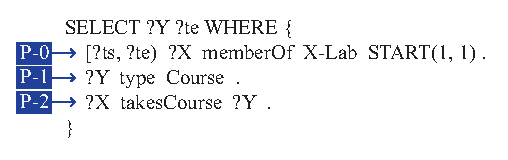
\includegraphics[width=0.55\textwidth]  {figures/trp.eps}}
\bicaption{显式指定使用“时序三元组存储”的查询语句示例}{Example of a query that explicitly specifies the use of "temporal triple storage"}
\label{trp}
\end{figure}

由于一条SPARQL-T查询语句可能包含多个五元模式或时序三元组时间范围模式,使用不同的顺序执行这些模式的效率可能不同,例如图\ref{trp}中的查询语句可以以以下两种不同的顺序执行:
\begin{itemize}
    \item 顺序一:
    \begin{itemize}
        \item 利用“时序三元组存储1”寻找变量\texttt{X}和\texttt{te}的所有可取值(P-0)
        \item 对于每行中间结果,从变量\texttt{X}的取值\texttt{val(X)}出发使用键\texttt{[val(X)| takesCourse|OUT]}找到变量\texttt{Y}的所有可取值(P-2)
        \item 对于每行中间结果,从变量\texttt{Y}的取值\texttt{val(Y)}出发使用键\texttt{[val(Y)| 1|OUT]}获取变量\texttt{Y}的类型,如果是\texttt{Course},则保留该行中间结果(P-1)
    \end{itemize}
    \item 顺序二:
    \begin{itemize}
        \item 利用“时序三元组存储1”寻找变量\texttt{X}和\texttt{te}的所有可取值(P-0)
        \item 使用键\texttt{[0|Course|IN]}找到变量\texttt{Y}的所有可取值(P-1)
        \item 对于每行中间结果,从变量\texttt{X}的取值\texttt{val(X)}出发使用键\texttt{[val(X)| takesCourse|OUT]}找到变量\texttt{Y}的可取值,如果其中包含变量\texttt{Y}的取值,则保留该行中间结果(P-2)
    \end{itemize}
\end{itemize}

由于系统并未实现SPARQL-T的执行优化器,无法自动确定最优的执行方案,所以需要用户在发起查询请求时通过自定义的查询计划指定查询引擎执行各模式的顺序。
另外,如果查询语句中包含时序三元组时间范围模式,查询引擎会先执行时序三元组时间范围模式,再执行五元模式。

SPARQL-T查询语句可分为大查询和小查询两类,大查询通常从大量顶点出发,探索庞大数量的路径,这一过程往往会访问时序RDF图中的很大一部分数据;小查询通常从一个固定的顶点开始,访问少量的路径和顶点。具体来说,大查询包含以下两类:
\begin{enumerate}
    \item 第一个查询模式需要用到键值对1-6的查询语句
    \item 包含时序三元组时间范围模式的查询语句
\end{enumerate}
其他的查询语句都属于小查询。

查询引擎使用fork-join机制来处理大查询。
工作线程在收到代理线程发来的大查询时,会将其分成\texttt{num\_qnodes} $\times$ \texttt{parallel\_factor}个子查询,然后分别发送给各个查询节点的\texttt{parallel\_factor}个工作线程共同执行,最后原工作线程负责子查询结果的合并。\texttt{parallel\_factor}是并行因子,其值越大,查询执行的并发度越高。

图\ref{fork-join}展示了一个大查询的fork-join过程,该查询的第一个查询模式需要使用键值对6。由于键值对6的值会被划分到所有查询节点存储,所以不同查询节点上读取到的键\texttt{[0|memberOf|IN]}对应的值是无共享的。同一查询节点上的不同工作线程读取到的值是相同的,工作线程会根据其线程号使用值列表中的一部分元素。
\begin{figure}[!htb]
\center{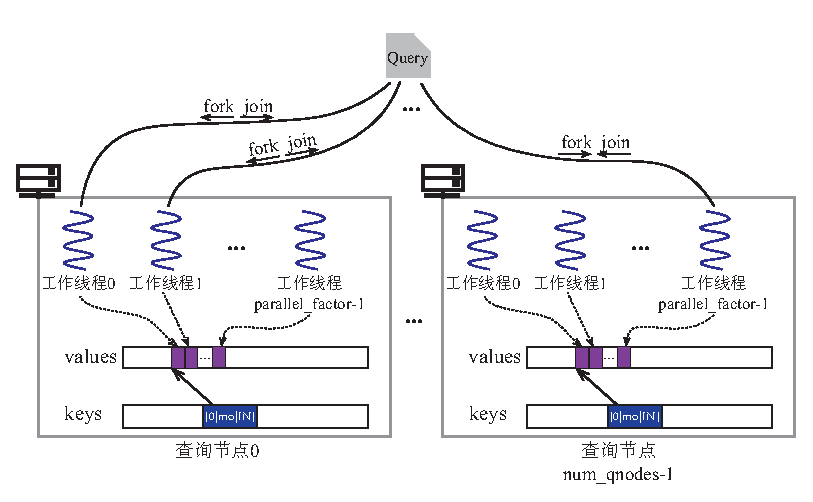
\includegraphics[width=0.75\textwidth]  {figures/fork-join.eps}}
\bicaption{大查询的fork-join过程}{Fork-join process of a heavy query}
\label{fork-join}
\end{figure}

查询引擎在处理小查询时也可能会使用fork-join机制:当工作线程在准备开始执行一个五元模式时,如果中间结果条目数达到系统预设的阈值(例如100),且工作线程需要通过较多跨节点的单边RDMA Read操作来执行该模式,那么工作线程会将其分成\texttt{num\_qnodes}个子查询,然后分别发送给各个查询节点的一个工作线程共同执行。查询的划分实质上是中间结果的划分,中间结果是依据执行该五元模式需要使用的变量的取值划分的,如果某行中间结果中该变量的取值为\texttt{val},那么该行中间结果会被划分到的子查询(从0开始编号)为:
\begin{equation}
    \mathtt{val \ \% \ num\_qnodes}
\end{equation}
查询划分完成后,子查询$i$会被发送到查询节点$i$执行。

只要遵守以上规则,子查询可以被进一步地划分,这样就可能形成一颗以代理线程发来的查询为根节点的查询树。

查询语句执行过程中,一个变量可能处于Unknown和Known两种状态,它们的含义分别为:
\begin{itemize}
    \item Unknown:该变量没有在之前的模式中出现过,当前中间结果表中没有该变量对应的列;
    \item Known:该变量已经在之前的模式中出现过,当前中间结果表中有该变量对应的列。
\end{itemize}

查询引擎在执行时序三元组时间范围模式时,会先从“时序超边存储”中查找所有符合模式指定的时间范围的时序三元组,然后逐一判断每个时序三元组是否与模式的前半部分(即\texttt{interval s p o})匹配。匹配一个时序三元组的方法为:先从\texttt{s}开始,如果它是变量且状态是Unknown,那么该时序三元组的主语就是它的一个可取值;如果它是变量且状态是Known,那么就需要逐一验证中间结果表每一行中该变量对应的列是否与该时序三元组的主语相同,若是则保留该行,否则舍弃该行;如果它是常量,那么只有在该时序三元组的主语与之相同时才可继续匹配。接着以类似过程匹配\texttt{p}、\texttt{o}、\texttt{interval}的\texttt{?var$_1$}和\texttt{?var$_2$}。

查询引擎在执行五元模式时,通常会先从其中的常量开始,通过构造合适的键从分布式键值存储中为模式中的变量寻找可取值,从而将变量的状态从Unknown转移到Known。然后可能会使用中间结果表每一行中Known变量对应的列的值继续构造合适的键进行进一步的图探索,直到所有五元模式都执行完毕。

\section{时序超图存储结构和查询引擎}
时序超图存储的设计思路与时序RDF图存储类似,都使用了分布式键值存储辅以分布式排序数组的存储结构。时序超图查询引擎使用存储层提供的接口逐一执行HQL-T查询语句中的各RP。本节将详细介绍时序超图的存储结构和查询引擎。
\subsection{存储结构}
\label{sec:hyperstore}
系统支持的时序超图数据集格式为\texttt{时序超边类型,时序超边名称,有效时间区间的开始时间,有效时间区间的截止时间,\{顶点名称1,顶点名称2,...\}}。
\sys 同样会将时序超图数据集中的字符串转化成整型ID进行存储。系统默认使用32位UINT表示顶点字符串对应的ID(下称\texttt{vid}),取值范围为$[2^{16}, 2^{32})$,对于顶点数量比较庞大的数据集,可以在系统编译时指定使用64位UINT表示\texttt{vid},取值范围就扩充到$[2^{16}, 2^{48})$。系统使用64位UINT表示时序超边ID(下称\texttt{heid}),取值范围为$[2^{16}, 2^{48})$。值得注意的是,可能有多条时序超边的名称相同,例如字符串“群聊1”可能对应多条时序超边,表示“群聊1”在不同时间区间下的成员情况。系统会给予相同名称的不同时序超边不同的\texttt{heid},在将表示时序超边名称的字符串转换成\texttt{heid}时,字符串服务器返回的是\texttt{heid}的列表。表示时序超边和顶点的类型的字符串对应的ID(下分别称\texttt{htid}和\texttt{tid})的范围为$[2,2^{16})$。

时序超图存储内存布局如图\ref{thyperstore},与时序RDF图存储类似,它分为键值存储区和时序超边存储区两部分。
时序超边存储区存储的是每个超边的ID、类型及其有效时间,即由\texttt{
[超边ID,超边类型,有效时间区间的开始时间,有效时间区间的截止时间]}四元组组成,它本质上也是内存数组。时序超边存储区分为两部分,在“时序超边存储1”中,四元组按照有效时间区间的开始时间升序排布;在“时序超边存储2”中,四元组按照有效时间区间的截止时间升序排布。时序超边的\texttt{heid}与它对应的四元组在“时序超边存储1”中的偏移量\texttt{off}的关系为:
\begin{equation}
    \mathtt{heid = off + 2^{16}}
\end{equation}
键值存储区中的键值对分为直接索引和间接索引两类,在直接索引中,值是实际数据;在间接索引中,值由指向“时序超边存储1”中四元组的指针组成。

\begin{figure}[!htb]
\center{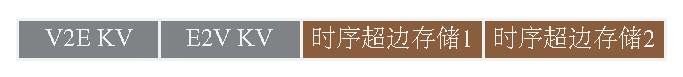
\includegraphics[width=0.6\textwidth]  {figures/thyperstore.eps}}
\bicaption{时序超图存储内存布局}{Temporal hypergraph storage memory layout}
\label{thyperstore}
\end{figure}

在键值存储区中,各种键值对及其类型如表\ref{tab:thyper}所示,系统使用两个分布式键值存储结构V2E KV和E2V KV来存储这些键值对。
键值对\ding{182}\textasciitilde\ding{184}位于E2V KV,键的数据类型是64位UINT,值的基本数据类型和\texttt{vid}的数据类型相同;键值对\ding{185}\textasciitilde\ding{188}位于V2E KV,键的数据类型也是64位UINT,由高48位和低16位两部分组成,值的基本数据类型是64位UINT。E2V KV中的键值对都是直接索引,V2E KV中的键值对除了\ding{185}外都是间接索引。
\begin{table}[!hpt]
  \bicaption{时序超图存储使用的键值对}{Key-value pairs used in temporal hypergraph storage}
  \label{tab:thyper}
  \centering
  \begin{tabular}{p{1cm}p{2cm}p{8cm}p{3cm}} \toprule
    序号 & 键 & 值 & 类型 \\ \midrule
    \ding{182}\centering & \texttt{[htid]} & 类型为\texttt{htid}的所有时序超边包含的所有\texttt{vid} & \multirow{4}{*}{直接索引} \\
    \ding{183}\centering & \texttt{[tid]} & 类型为\texttt{tid}的所有\texttt{vid} & \\
    \ding{184}\centering & \texttt{[heid]} & 时序超边\texttt{heid}包含的所有\texttt{vid} & \\
    \ding{185}\centering & \texttt{[vid|0]} & 顶点\texttt{vid}的\texttt{tid} & \\ 
    \hline
    \ding{186}\centering & \texttt{[vid|htid]} & 包含顶点\texttt{vid}且类型为\texttt{htid}的所有时序超边 & \multirow{2}{*}{间接索引} \\ 
    \ding{187}\centering & \texttt{[0|htid]} & 类型为\texttt{htid}的所有时序超边 & \\ 
    \bottomrule
  \end{tabular}
\end{table}

图\ref{thsdemo}(a)展示了一个简单的时序超图拓扑,它从微信中的群聊及公众号和微信用户之间的关系抽象而来,它包含两类时序超边:群聊成员和公众号关注者。
有两条类型为群聊成员的时序超边:“群聊1”、“群聊2”,有三条类型为公众号关注者的时序超边:“公众号1”、“公众号2”、“公众号3”,有10个名称分别为A\textasciitilde J的类型为微信用户的顶点。
图\ref{thsdemo}(b)给出了系统会为其生成的一部分键值对。为了便于理解,图中使用字符串表示时序超边、顶点及其类型,系统实际使用的是这些字符串对应的ID。
在间接索引中,值是一个由时序超边对应的四元组在“时序超边存储1”中的偏移量组成的列表,例如,时序超边“群聊2”对应的四元组在“时序超边存储1”中的偏移量为1,那么间接索引就使用1来表示“群聊2”。

\begin{figure}[!htb]
\center{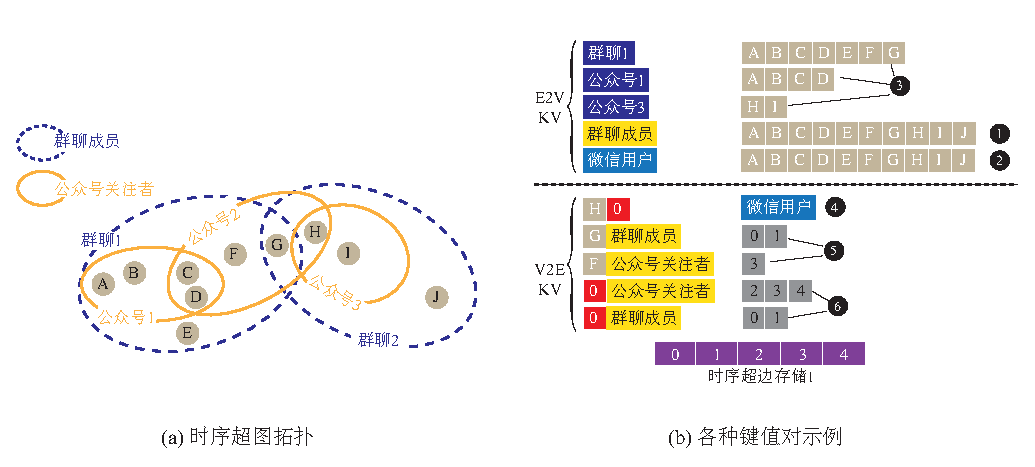
\includegraphics[width=0.95\textwidth]  {figures/thsdemo.eps}}
\bicaption{时序超图存储使用的键值对示例}{Example of key-value pairs used in temporal hypergraph storage}
\label{thsdemo}
\end{figure}

为了实现分布式可扩展存储,系统使用如下规则将键值对和时序超边划分到各查询节点中存储:
\begin{enumerate}
    \item \label{partitionRule1} 每个查询节点负责一块连续ID的时序超边和顶点的管理,时序超边\texttt{heid}会被分配到的查询节点(查询节点从0开始编号)为:
    \begin{equation}
        \mathtt{(heid - 2^{16}) \ / \ \lceil num\_thes \ / \ num\_qnodes \rceil}
    \end{equation}
    其中\texttt{num\_thes}是时序超边总数,\texttt{num\_qnodes}是查询节点数。顶点的分配方法同理。
    \item 对于键值对\ding{182}\ding{183}\ding{187},将值按照\ref{partitionRule1}中的规则划分到各查询节点存储,同一键会出现在每个查询节点的键值存储中;对于键值对\ding{184}\ding{185}\ding{186},将键依据其高48位按照\ref{partitionRule1}中的规则划分到不同查询节点存储,每个键只会出现在一个查询节点的键值存储中。
    \item 将所有四元组分别按有效时间区间的开始时间和截止时间排序后,分别按块划分到各查询节点的“时序超边存储1”和“时序超边存储2”中存储,偏移量为\texttt{off}的四元组会被分配到的查询节点(从0开始编号)为:
    \begin{equation}
        \mathtt{off \ / \ \lceil num\_thes \ / \ num\_qnodes \rceil}
    \end{equation}
\end{enumerate}

\subsection{查询引擎}
HQL-T查询引擎同样沿用了Wukong使用的图探索和全历史剪枝算法。默认情况下,查询引擎会使用存储层提供的接口通过键值存储查找所需的数据,但对于一些以时间点或时间范围为条件的查询,直接在“时序超边存储”上通过二分法查找符合条件的时序超边可能更加高效。例如图\ref{hql}中的查询语句是要查找最后一次成员变动发生于2023年10月1日到2023年10月7日期间的所有群聊及其成员,在执行该语句时,可以使用“时序超边存储1”快速找到有效时间区间开始时间在2023年10月1日到2023年10月7日期间的所有时序超边,然后从中筛选出类型为“群聊成员”且有效时间区间截止时间晚于当前时间的时序超边即可。如果查询引擎不使用“时序超边存储”,而是先从键值存储中找到所有类型为“群聊成员”的时序超边,再筛选出有效时间区间符合条件的时序超边,那么就会带来更大的数据访问开销。目前系统尚未实现HQL-T的查询优化器,无法自动判断使用键值存储和使用“时序超边存储”哪个效率更高。系统的替代方案是将选择权交给用户,由用户在查询语句中使用\textbf{时序超边时间范围模式}显式地指定使用“时序超边存储”进行时间条件查询,语法为:
\begin{equation}
    \mathtt{?var \ STRAT/END(const_1, const_2) \ interval}
\end{equation}

其中变量\texttt{?var}会取值为查询到的时序超边的\texttt{heid};\texttt{START}和\texttt{END}二选一,\texttt{START}指定依据有效时间区间开始时间进行查找,\texttt{END}指定依据有效时间区间截止时间进行查找;\texttt{const$_1$}和\texttt{const$_2$}是两个时间常量且\texttt{const$_1\leq$const$_2$},用于指定要查找的时间范围;\texttt{interval}是可选的,它是一个由两个变量组成的区间,格式为\texttt{[?var$_1$,?var$_2$)},当它存在时,两个变量会分别取值为查询到的时序超边的有效时间区间的开始时间和截止时间。我们规定,时序超边时间范围模式只能出现在GP中最开始的位置,它们会先于RP被处理。值得注意的是,用户需要自行估算使用时序超边时间范围模式是否能够提高查询的执行效率,避免出现负优化。图\ref{guide}中的查询语句与图\ref{hql}中的查询语句含义相同,但它显式地指定使用“时序超边存储1”进行时间范围查询。

\begin{figure}[!htb]
\center{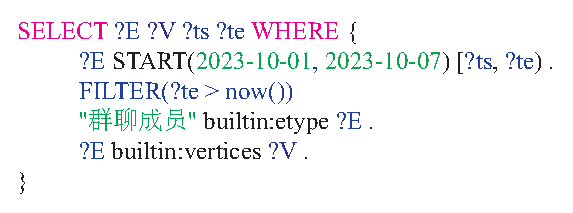
\includegraphics[width=0.55\textwidth]  {figures/guide.eps}}
\bicaption{显式指定使用“时序超边存储”的查询语句示例}{Example of a query that explicitly specifies the use of "temporal hyperedge storage"}
\label{guide}
\end{figure}

与SPARQL-T类似,HQL-T查询语句同样可分为大查询和小查询两类,大查询通常以大量时序超边或顶点作为起始,然后探索更多数量的时序超边和顶点;小查询通常从一个固定的时序超边或顶点开始,访问少量的时序超边和顶点。具体来说,大查询包含以下两类:
\begin{enumerate}
    \item 第一个查询模式是GE或GV模式的查询语句;
    \item 包含时序超边时间范围模式的查询语句。
\end{enumerate}
其他的查询语句都属于小查询。
查询引擎同样使用fork-join机制来处理大查询,其过程与SPARQL-T查询引擎完全相同,在此不作赘述。

查询引擎在处理小查询时同样可能会使用fork-join机制:当工作线程在准备开始执行一个RP时,如果中间结果条目数达到系统预设的阈值(例如100),且工作线程需要通过较多跨节点的单边RDMA Read操作来执行该RP,那么工作线程会将其分成\texttt{num\_qnodes}个子查询,然后分别发送给各个查询节点的一个工作线程共同执行。在划分查询时,中间结果是依据输入元素列表中的第一个变量的取值划分的,如果某行中间结果中该变量的取值为\texttt{val},那么该行中间结果会被划分到的子查询(从0开始编号)为:
\begin{equation}
    \mathtt{(val - 2^{16}) \ / \ \lceil num\_thes \ / \ num\_qnodes \rceil}
\end{equation}

V2E、E2V、V2V和E2E这四种RP的执行比较复杂,执行这些模式时输入元素列表中各变量的状态一定是Known,输出元素列表中变量的状态是Known或Unknown。接下来我们分别详细介绍这四种RP的执行逻辑,我们只讨论输出元素列表中变量的状态是Unknown的情况;对于V2E、E2V和E2E模式,我们只讨论包含\texttt{interval}的情况。
\begin{itemize}
    \item \textbf{V2E模式:}该模式的输入元素列表可以包含若干表示顶点的常量或变量。执行该模式时,首先需要使用键值对\ding{186}分别获取输入元素列表中的各常量对应的\texttt{heid}集合,然后求取这些集合的交集$s_1$。接下来对于每行中间结果,再使用键值对\ding{186}分别获取输入元素列表中各变量取值对应的\texttt{heid}集合,求取这些集合的交集$s_2$,然后求取$s_1$和$s_2$的交集$s$,$s$即是该变量可取值的集合。最后根据\texttt{heid}计算出偏移量,在“时序超边存储1”中读取对应四元组中的生命周期信息即可。
    \item \textbf{E2V模式:}该模式的输入元素列表可以包含若干表示时序超边的常量或变量。输入元素列表中的一个常量可能对应多条时序超边,查询引擎需要首先计算能够使得每个常量对应的时序超边都有且仅有一个有效的所有时间区间,记为$itv_1, itv_2,...,itv_n$(在图\ref{e2v}中是红色虚线标出的三个时间区间),然后对于每一个时间区间,使用键值对\ding{184}分别获取每条有效的时序超边对应的\texttt{vid}集合并求交集,记得到的集合为$s_1, s_2, ..., s_n$。接下来对于每行中间结果,计算能够使得输入元素列表中各变量取值表示的时序超边都有效的最大时间区间,记为$itv$(在图\ref{e2v}中是黑色虚线标出的时间区间,由于每个变量的取值只能表示一条时序超边,所以此处最多计算得到一个时间区间),然后使用键值对\ding{184}分别获取这些时序超边对应的\texttt{vid}集合,求取这些集合的交集$s$,最后将时间区间$itv$分别与时间区间$itv_1, itv_2,...,itv_n$求交,得到新的时间区间$itv_1', itv_2',...,itv_m'$(在图\ref{e2v}中是黑色双向箭头标出的两个时间区间)并计算每个新时间区间上$s_i$和$s$的交集$s_i'$。最终,一行中间结果能够生成$|s_1'|+|s_2'|+...+|s_m'|$行新的中间结果。
    
    \begin{figure}[!htb]
    \center{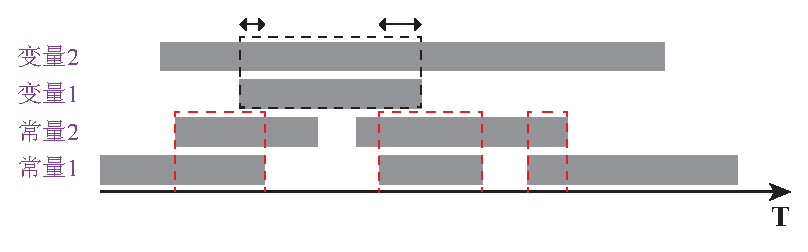
\includegraphics[width=0.6\textwidth]  {figures/e2v.eps}}
    \bicaption{执行E2V模式时对时间区间的处理过程}{Processing of time intervals when executing E2V pattern}
    \label{e2v}
    \end{figure}
    
    \item \textbf{V2V模式:}该模式的输入元素列表可以包含若干表示顶点的常量或变量。执行该模式时,首先要为输出元素列表中的变量寻找候选取值,为此,查询引擎将包含输入元素列表中第一个常量(如果输入元素列表没有常量,则是第一个变量的取值)所表示的顶点的所有时序超边包含的所有顶点作为候选顶点集合。确定候选顶点集合后,查询引擎会逐一验证每个候选顶点是否同时与各输入顶点出现在相同时序超边且时序超边的数量满足参数的要求,验证通过的候选顶点才会作为输出元素列表中变量的取值。
    \item \textbf{E2E模式:}该模式的执行逻辑与E2V模式的执行逻辑相似,此外,执行此模式同样需要为输出元素列表中的变量寻找候选取值,然后验证候选取值是否能够使得参数指定的条件成立。该模式的详细执行过程不再赘述。
\end{itemize}

\section{本章小结}
本章介绍了\sys 时序图查询模块的设计与实现。时序RDF图和时序超图都没有标准的查询语言,所以本文在RDF图查询语言SPARQL的基础上设计了时序RDF图查询语言SPARQL-T,从零开始设计了时序超图查询语言HQL-T。SPARQL-T将SPARQL的GP中的三元模式扩展到五元模式,HQL-T的GP则由基础关系模式(RP)组成。时序RDF图存储和时序超图存储的设计思路类似,都使用了分布式键值存储辅以分布式排序数组的存储结构,键值存储都使用了直接索引和间接索引相结合的设计,在实现了高效的拓扑查询和时间条件查询的同时,减少了时序数据存储占用的空间。
SPARQL-T的时序三元组时间范围模式和HQL-T的时序超边时间范围模式可以用来在特定条件下加速时间条件查询。
SPARQL-T和HQL-T查询引擎都沿用了Wukong使用的图探索和全历史剪枝算法,都使用了fork-join机制来加速复杂查询的执行。

\chapter{时序图分析模块的设计与实现}
\sys 的时序图分析模块运行在一个单独的分析节点上,同时处理图事务请求和第一类时序图分析任务,它包含的时间数据属于事务时间。
本章将详细介绍一个高效可更新的、基于时序属性图模型的图存储结构\store,然后介绍时序图分析模块使用的基于epoch的粗粒度MVCC机制和\store 结合该机制的修改后版本\newstore,分析这些优化是如何带来读写效率的提升的。
最后将介绍时序图分析模块的只读事务,以及如何基于只读事务在图分析引擎中实现时序图分析算法。

\section{动态图存储结构\store}
图拓扑的CSR表示具有非常好的读性能,但它更新起来非常困难;邻接列表表示的更新效率更高,但它会牺牲读的性能。
为了在实现时序图分析模块的高效图分析性能的同时,保证其良好的图更新效率,本文设计了一个高效的动态图存储\store,它实现了与CSR接近的良好的数据局部性,同时也支持高效的图数据更新。

\begin{figure}[htb]
\center{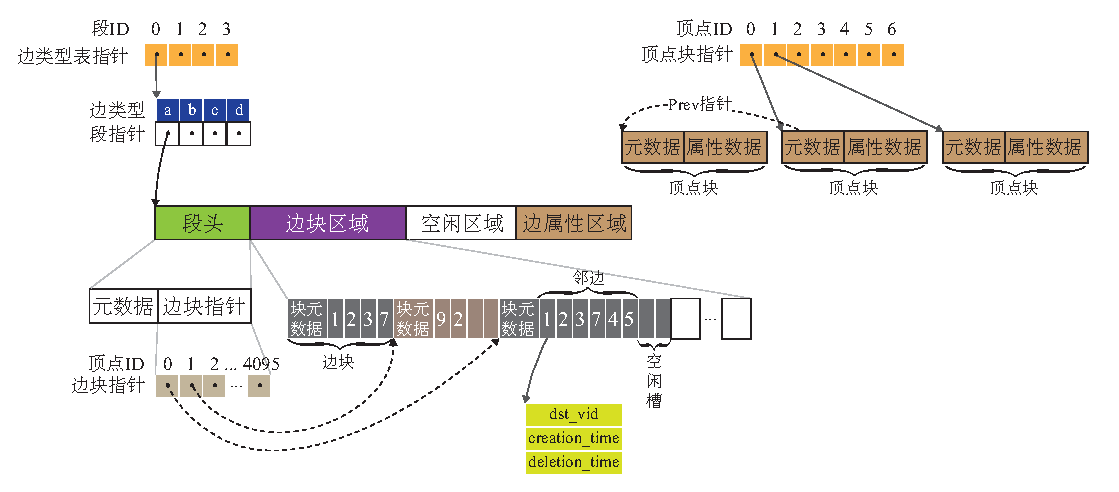
\includegraphics[width=1\textwidth]  {figures/segcsr.eps}} 
\bicaption{动态图存储\store 的结构}{The structure of dynamic graph storage \store}
\label{segcsr}
\end{figure}

\store 的结构如图\ref{segcsr}。\store 使用段来管理固定数量(默认 4096)顶点的所有特定类型的邻边,如果使用\texttt{Seg(sid,type)}表示ID为\texttt{sid}、管理的邻边类型为\texttt{type}的段,那么段\texttt{Seg(0,a)}管理的是ID为 $0-4095$的顶点的所有类型为\texttt{a}的邻边,段\texttt{Seg(1,b)}管理的是ID为$4096-8191$的顶点的所有类型为\texttt{b}的邻边。
\store 使用边类型表\texttt{ETT(sid)}来维护段ID为\texttt{sid}的管理不同邻边类型的段的地址,边类型表的每个表项都是一个边类型到段地址的映射。\store 使用一个边类型表地址数组来维护各边类型表的地址。

一个段由四部分组成,分别是段头、边块区域、空闲区域和边属性区域。段的初始大小是固定的(例如1MB)。段头由两部分组成:段的元数据和指向各顶点边块的指针。段的元数据包括段ID、段大小和已使用段空间大小等。在一个段中,每个顶点都对应一个最新的边块。边块是一块连续的内存区域,由块元数据和边数据区两部分组成。块的元数据包括顶点ID、块大小和已使用块空间大小等。边数据区由描述边信息的结构体组成,该结构体包含三个字段,dst\_vid是边的终点ID,creation\_time是该边的创建时间,deletion\_time是该边的删除时间,它的默认值是INT64\_MAX,表示它还未被删除。边块的初始大小固定,最初被分配出来时会有若干空闲槽,供后续边的插入。如果在插边时发现目标边块的空闲槽已经被用尽,分配器会从空闲区域里分配一个大小为目标边块2倍的新边块,然后把原边块里的数据都迁移到这个新边块里,之后相应顶点的邻边会插入这个新边块中。段头中每个顶点的边块指针指向的是其最新的边块。边块是自段头开始从左往右分配的,而边属性区域是自段尾开始从右往左增长的,边块区域里的边和边属性区域里的边属性数据是对称排布的(如图\ref{edge_property}),块元数据中包含该边块里的边的属性数据在边属性区域中的起始位置。我们要求一个段中各边的属性数据大小相同,以便能够为边块中的空闲槽预留边属性存储空间。

\begin{figure}[htb]
\center{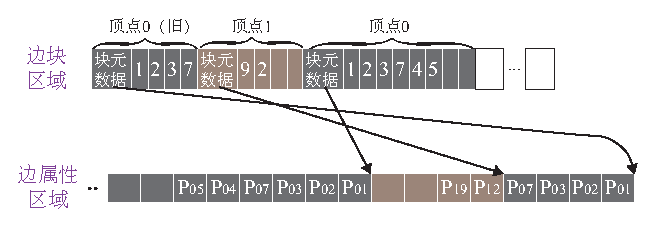
\includegraphics[width=0.7\textwidth]  {figures/edge_property.eps}}
\bicaption{边和边属性数据的对称排布}{Symmetrical layout of edge and edge property data \store}
\label{edge_property}
\end{figure}

如果段的空闲区域不足以分配出新边块和边属性存储空间时,分配器会启动段的迁移过程:分配一个大小为原段二倍的新段,然后按照顶点ID的顺序把原段中每个顶点最新的边块和对应的边属性数据复制到新段里并更新每个顶点的边块指针,最后修改边类型表里的相应地址为新段的地址。

\store 使用顶点块来存储顶点的属性数据,顶点块由元数据区和属性数据区两部分组成,元数据区包含顶点ID、属性数据大小、顶点创建时间和旧顶点块指针等。顶点属性数据更新时,新的顶点块会被创建,其元数据中的旧顶点块指针会指向较旧版本的顶点块,形成一个由不同版本的顶点块组成的链表结构。\store 使用一个顶点块地址数组来维护每个顶点的最新版本顶点块的地址。

\store 使用一个段来管理一定数量的顶点的所有特定类型的邻边,这使得同属于一个段的顶点的边块之间和邻边的属性数据之间都不会离得太远,大大提高了扫边时的数据局部性,从而显著提高扫边性能。段的空闲空间不足时的段迁移操作会按照顶点ID的顺序把原段中每个顶点的边块和邻边的属性数据复制到新段里,使得新段达到近似于CSR的瞬时数据局部性。

绝大多数的并发写问题都可以通过原子操作来解决,例如边块的并发分配可以通过对段头元数据中的已使用段空间大小字段的原子写来实现,对同一边块的并发插入可以通过对块元数据中的已使用块空间大小字段的原子写来实现。
但以下两种并发问题需要使用锁来解决:
\begin{enumerate}
    \item \label{para1} 段迁移过程中的并发问题。考虑以下场景:事务A和事务B在同时往段S中插边,事务A的目标边块有空闲槽,事务B的目标边块没有空闲槽,且段S的空闲区域不足以分配出一个新边块,这时分配器就要为事务B启动段S的迁移,如果段迁移时事务A还未提交(假设系统保证了快照隔离),那么迁移后的段就会丢失事务A插入的边。为了解决这种并发冲突,系统引入了段级别的读写锁:普通的边更新操作只需要尝试获取段的共享锁(读锁),而当该边更新操作会触发段的迁移时,它就会尝试获取段的互斥锁(写锁)。
    \item 边块迁移过程中的并发问题。该问题与\ref{para1}类似,系统使用顶点级别的互斥锁来解决这种并发冲突:边更新操作需要尝试获取起点的互斥锁。
\end{enumerate}

\section{粗粒度的MVCC机制}
MVCC (multi-version concurrency control,多版本并发控制)是一种实现数据库的并发读写的常用方法,它能够避免读操作造成的写操作的阻塞,当数据库中的某个数据值被更新时,MVCC会为该值创建一个新版本,使得并发的读操作可以读到一个稳定的版本。
\store 使用两个时间戳creation\_time和deletion\_time分别表示边的创建时间和删除时间,使用时间戳creation\_time表示顶点的创建时间并使用链表结构将不同版本的顶点块组织起来,以此来实现MVCC。
实时图处理系统通常使用细粒度的MVCC机制,例如LiveGraph使用了组提交策略\cite{grpcmt},每次提交都会将全局写版本号加1,事务的本地写版本号是事务开始时的全局写版本号,它会被用于标识事务所操作数据的版本号。
在图分析场景中,细粒度的MVCC机制是不必要的:图分析是一类相对繁重的计算任务,其执行时间要远远超过一个图事务的执行时间,无需为每次图事务的提交都准备一个不同的版本号,因为图分析任务对细粒度的版本号并不敏感。

为了减少版本数据带来的内存使用和额外计算开销,系统使用了一种基于epoch的粗粒度MVCC机制。
系统会维护一个全局的epoch ID,它从0开始,每隔几十微秒递增一次。
如图\ref{epoch},两个相邻的epoch之间的屏障会使得上一个epoch中的所有事务都完成时,才会开始下一个epoch中事务的执行。
事务的本地写版本号就是其所在epoch的ID,它会被用于标识事务所更新数据的版本号。
同一epoch中的事务可以并行执行,图更新引擎会保证这些事务不会有依赖关系(有依赖关系的事务会按照串行顺序被分配到不同的epoch中执行)。
系统管理员在发起时序图分析任务时需要指定读版本号,时序图分析能够使用的最新稳定版本是\texttt{ceid-1},其中\texttt{ceid}是系统当前的epoch ID。
 
\begin{figure}[htb]
\center{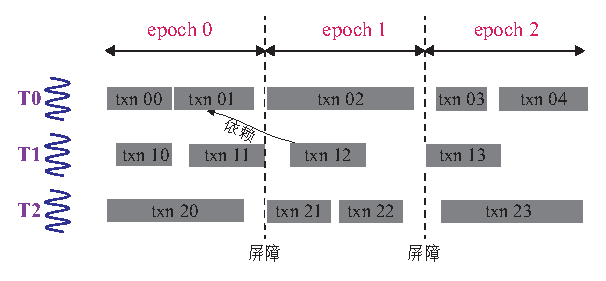
\includegraphics[width=0.6\textwidth]  {figures/epoch.eps}}
\bicaption{epoch屏障示例}{epoch barrier example}
\label{epoch}
\end{figure}

基于上述MVCC机制,我们对\store 的结构进行了调整,使其充分从新的MVCC机制受益,调整后的存储结构称为\newstore。
\newstore 的结构如图\ref{newseg},与\store 相比,它将边块中描述边信息的结构体简化为只包含表示边终点ID的dst\_vid,边块中各边的版本信息(即添加各边的事务的本地写版本号)被统一存储在一个epoch表中。
系统会为段管理的每个顶点都分配一块连续内存作为epoch表,epoch表负责维护顶点的最新边块里的所有边的版本信息,段头会存储每个顶点的epoch表的地址。
边块中的边是只追加的(append-only),相同版本号的边会连续存储,epoch表存储的是每个epoch里添加的第一条边在边块里的逻辑偏移量,例如图\ref{newseg}中顶点0的epoch表的含义就是偏移量为0\textasciitilde 1的边是在epoch 0被插入的,偏移量为2\textasciitilde 4的边是在epoch 3被插入的,偏移量为$5$的边是在epoch 4被插入的。

\begin{figure}[htb]
\center{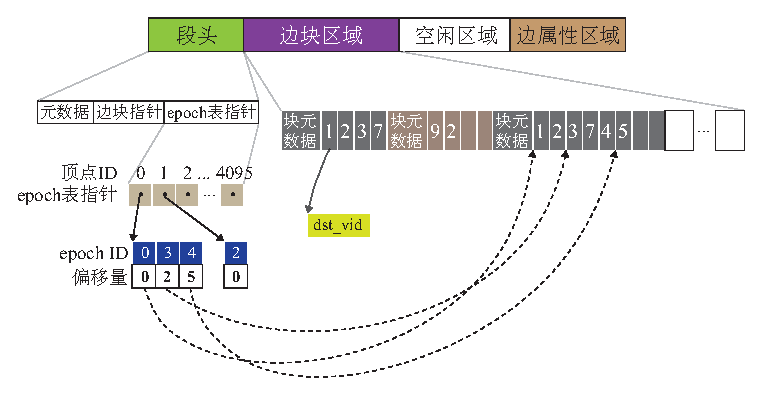
\includegraphics[width=0.9\textwidth]  {figures/newseg.eps}}
\bicaption{\newstore 的结构}{The structure of \newstore}
\label{newseg} 
\end{figure}


\textbf{边的插入。}假设要插入的边是$(u, v)$,其类型为$ty$。
首先通过边类型表地址数组找到边类型表,然后在边类型表中查找类型$ty$对应的表项,即为目标段的地址。
接下来通过目标段的段头中顶点$u$的边块地址即可定位到目标边块,如果目标边块还有空闲槽,则直接把$v$插入第一个空闲槽即可,否则启动边块的迁移,然后再把$v$插入新边块的第一个空闲槽。
边的属性数据要插入边属性区域中的对称位置,相关的元数据(例如块元数据中已使用块空间大小等)也要更新。
如果事务的epoch ID已经存在于顶点$u$对应的epoch表中,则epoch表无需改变,否则需要在epoch表中增加一个表项\texttt{<teid,off>},其中\texttt{teid}就是事务的epoch ID,\texttt{off}是$v$在边块中的偏移量。

\textbf{边的删除。}由于边块中的边数据是只追加的,所以边的删除需要通过边数据的添加来实现。
使用同样的方法定位到目标边块后,通过在边块中添加一个删除标记来记录被删除的边在边块中的偏移量。如果在图分析的扫边过程中遇到删除标记,被删除的边会被直接跳过。

\textbf{垃圾回收。}后台的垃圾回收线程负责过时数据的清理,\newstore 的过时数据包括:
\begin{itemize}
    \item 旧段。段迁移完成后,新段的地址会被注册到边类型表,后续段寻址就会被转移到新段。由于旧段上可能还有未完成的读,所以旧段不能在段迁移完成后就被立即回收。
    垃圾回收线程会监控旧段的使用,旧段上的所有读都完成后,垃圾回收线程就会将其回收。
    \item 被删除的边。为了实现边块的只追加性,系统使用删除标记来记录边的删除。后台的垃圾回收线程会定期对边块中的删除标记进行整理,将删除标记和对应的被删除的边物理地从边块移除。
\end{itemize}

\section{时序图分析算法的实现}
时序图分析模块提供了只读事务RO\_TXN,时序图分析算法都是基于RO\_TXN实现的。表\ref{tab:rotxn}给出了与RO\_TXN相关的接口。

\begin{table}[!hpt]
  \bicaption{RO\_TXN相关接口}{RO\_TXN related interfaces}
  \label{tab:rotxn}
  \centering
  \begin{tabular}{p{7cm}p{5cm}p{2cm}} \toprule
    接口 & 作用 & 类型 \\ \midrule
    \texttt{ROTxn begin\_ROTxn(reid)} & 创建一个读epoch ID为\texttt{reid}的只读事务 & \newstore 的成员函数 \\
    \hline
    \texttt{Seg* locate\_seg(sid,etype)} & 定位段\texttt{Seg(sid,etype)} & \multirow{3}{2cm}{ROTxn的成员函数} \\
    \texttt{EdgeIter get\_edges(segptr,vid)} & 获取地址为\texttt{segptr}的段中顶点\texttt{vid}的邻边的迭代器 \\
    \texttt{sid\_t max\_sid get\_max\_sid()} & 获取最大的段ID \\
    \hline
    \texttt{bool valid()} & 迭代器是否迭代完毕  & \multirow{5}{2cm}{EdgeIter的成员函数} \\
    \texttt{void next()} & 迭代到下一条边 \\
    \texttt{vertex\_t dst\_id()} & 当前边的终点ID \\
    \texttt{string edge\_data()} & 当前边的属性数据 \\
    \texttt{size\_t size()} & 剩余未迭代到的边的数量 \\
    \bottomrule
  \end{tabular}
\end{table}

算法\ref{algo:anademo}使用这些接口实现了一个简单的时序图分析算法,它扫描版本(epoch ID)\texttt{reid}下所有顶点的所有有效邻边,同时把边的属性数据打印出来。首先需要通过begin\_ROTxn接口创建一个读epoch ID为\texttt{reid}的只读事务(第1行),然后使用RO\_Txn提供的get\_max\_sid接口获取该版本下最大的段ID(第2行),接着逐个遍历每个段(3-12行)。在遍历一个段的过程中,需要逐一扫描该段管理的每个顶点的边块:通过RO\_Txn提供的get\_edges接口获取顶点邻边的迭代器(第7行),依次打印迭代到的每条边的属性数据即可(8-12行)。

\begin{algorithm}[htb]
\caption{一个简单的时序图分析算法的实现}
\label{algo:anademo}
\SetKw{KwIn}{in}
\SetKw{KwTo}{to}
\SetKwFunction{Range}{range}
\SetKwFor{For}{for}{\string:}{}
\SetKwIF{If}{ElseIf}{Else}{if}{:}{elif}{else:}{}
\SetKwFor{While}{while}{:}{}
\newcommand{\forcond}{sid = 0 \KwTo{max\_sid}}
\newcommand{\forcondtype}{etype \KwIn{etypes}}
$txn$ = $graph$.begin\_ROTxn($reid$)\;
$max\_sid$ = txn.get\_max\_sid()\;
\For{\forcond}{
    \For{\forcondtype}{
        $segptr$ = txn.locate\_seg($sid$,$etype$)\;
        \For{$vid$ = $sid$ * NUM \KwTo{($sid$ + 1) * NUM - 1}}{
            $iter$ =  $txn$.get\_edges($segptr$,$vid$)\;
            \While{$iter$.valid()}{
                $dst\_id$ = $iter$.dst\_id()\;
                $data$ = $iter$.edge\_data()\;
                print($data$)\;
                $iter$.next()\;
            }
        }
    }
}
\end{algorithm}

目前,时序图分析模块已经实现了多种常用的图分析算法,包括广度优先搜索(BFS)、PageRank、单源最短路径(SSSP)和强连通分量(SCC)等。

\section{本章小结}
本章介绍了\sys 时序图分析模块的设计与实现。系统的时序图分析模块使用了一个高效可更新的、基于时序属性图模型的图存储结构\newstore,它使用段(一块连续的内存空间)来管理固定数量顶点的所有特定类型的邻边,这使得同属于一个段的顶点的边块之间和邻边的属性数据之间都不会离得太远,大大提高了扫边时的数据局部性,从而显著提高扫边性能。为了减少时序数据带来的内存使用和额外计算开销,\newstore 使用了一种基于epoch的粗粒度MVCC机制。最后,时序图分析模块提供了只读事务RO\_TXN,时序图分析算法都是基于 RO\_TXN实现的。
\chapter{实验与评测}
\sys 是一个高效的时序图处理系统,为了检验系统的性能,本文设计了一系列实验从多个角度对系统的性能进行全面的评测。
本章将对各实验的设计和结果进行详细的介绍,并给出各实验数据的详细分析。

\section{实验配置}
\noindent\textbf{实验环境}\ 系统运行在一个由8台机器组成的集群中,其中一台机器用作字符串服务器节点,一台机器运行分析节点,其余6台机器运行查询节点。每台机器都配备了两个Intel Xeon E5-2650 CPU,每个CPU都有8个核心、16个超线程。每台机器的内存都是128GB,都配备一张Mellanox
ConnectX-5 100Gbps InfiniBand网卡。8台机器通过一台Mellanox 100Gbps InfiniBand交换机互联。
所有机器运行的操作系统都是Ubuntu 16.04 (4.15.0-46-generic),InfiniBand网卡驱动为MLNX\_OFED\_LINUX-4.9-3.1.5.0。
其他软件版本为gcc/g++ v7.4.0、cmake v3.22.0和Python v3.8。

\noindent\textbf{使用的数据集}\ 实验使用的RDF数据集是开源项目LUBM\cite{lubm}生成的数据集。LUBM是里海大学发布的用于评测RDF数据集管理系统的查询性能的基准测试项目,LUBM数据集描述了大学里各种实体之间的关系,例如学生、教师、学院和课程等。生成数据集时,可以通过指定数据集包含的大学的数量来设置生成的数据集的规模,实验使用的数据集是LUBM 10240,它包含337M个实体,1410M个三元组。
LUBM数据集本身不包含时序数据,我们为每个三元组都随机生成了两个64位INT型时间戳$t_1$和$t_2$($t_1<t_2$,时间戳是从1970-01-01T00:00:00Z开始经过的秒数),分别表示三元组有效时间区间的开始时间和截止时间,得到的时序数据集称为tLUBM 10240。

实验使用的时序超图数据集是一个现实的金融数据集FIN,它描述了金融领域中的上市公司、基金、客户和供应商等之间的关系,包含661K条时序超边和360K个顶点。

图存储结构\store 和\newstore 的微观性能评测使用了LDBC SNB\cite{snb}、Wiki\cite{wiki}、R-MAT\cite{rmat}、UK-2005\cite{uk}和Twitter-2010\cite{twitter}5个图数据集。
LDBC SNB是一个图分析系统的基准测试项目,它包含一个社交网络图数据集生成器和多种图分析工作负载。
LDBC SNB数据集是一个描述社交网络中人、论坛、帖子和评论等实体之间关系的图,在生成数据集时,可以通过指定规模因子 (scale factor, SF)来控制生成的数据集的大小,实验使用的数据集SF=10。Wiki、R-MAT、UK-2005和Twitter-2010都是现实的图数据集。5个图数据集的统计信息见表\ref{tab:dataset}。

时序图分析模块的事务处理性能和图分析性能评测使用的是LDBC SNB (SF=10)基准测试,数据集会通过数据生成器提前生成,所有顶点和50\%的边会被批量加载到系统中,剩余50\%的边会通过客户端发起的图更新事务插入到系统中。

\begin{table}[!hpt]
  \bicaption{LDBC SNB (SB)、Wiki (WK)、R-MAT (RM)、UK-2005 (UK)和Twitter-2010 (TW) 5个图数据集的统计信息}{Statistics of 5 graph datasets: LDBC SNB (SB), Wiki (WK), R-MAT (RM), UK-2005 (UK) and Twitter-2010 (TW)}
  \label{tab:dataset}
  \centering
  \begin{tabular}{p{2cm}p{1cm}p{1cm}p{1cm}p{1cm}p{1cm}} \toprule
    \textbf{图数据集}\centering & \textbf{SB} & \textbf{WK} & \textbf{RM} & \textbf{UK} & \textbf{TW} \\ \midrule
    |V|\centering & 7.5M & 5.7M & 5.0M & 39.5M & 41.7M \\
    |E|\centering & 8.8M & 130M & 300M & 936M & 1.47B \\
    \bottomrule
  \end{tabular}
\end{table}

\noindent\textbf{实验基准}\
为了评测系统处理时序RDF图查询的性能,我们将\sys 与NebulaGraph和Neo4j两个系统进行了对比。
NebulaGraph和Neo4j都是基于属性图模型的图数据库,NebulaGraph支持分布式的存储和图查询处理,而Neo4j是单机图数据库。为了实现NebulaGraph和Neo4j对tLUBM 10240数据集的存储,我们将tLUBM 10240通过表\ref{tab:rdf2prop}中列出的映射转换为属性图数据集。NebulaGraph和Neo4j支持的图查询语言分别是nGQL和Cypher,SPARQL-T查询语句都可以转换成这两种查询语言。

\begin{table}[!hpt]
  \bicaption{时序RDF图到属性图的映射}{Mapping from temporal RDF graph to property graph}
  \label{tab:rdf2prop}
  \centering
  \begin{tabular}{p{8cm}p{7cm}} \toprule
    \textbf{时序RDF图} & \textbf{属性图} \\ \midrule
    时序三元组中的主语和宾语(表示类型名的宾语除外) & 顶点名 \\
    表示类型名的宾语 & 顶点类型 \\
    时序三元组中的主语、谓词和宾语(描述主语类型的时序三元组除外) & 主语对应的顶点指向宾语对应的顶点的有向边,边的类型是谓词 \\
    时序三元组中的有效时间区间(描述主语类型的时序三元组除外) & 对应边的两个属性 \\
    描述主语类型的时序三元组的有效时间区间 & 主语对应的顶点的两个属性 \\
    \bottomrule
  \end{tabular}
\end{table}

由于超图查询系统相关研究工作很少,所以我们并没有找到合适的基准时序超图查询系统来与\sys 作对比,我们的方案是将与时序超图数据集FIN等价的时序RDF图数据集加载到\sys 的时序RDF图存储中,然后通过等价的HQL-T和SPARQL-T查询语句来对比在查询等价数据时,\sys 的时序超图查询的性能和时序RDF图查询的性能。将时序超图数据集转换为时序RDF图数据集的方法为:将类型为\texttt{ty}、名称为\texttt{name}、连接$n$个顶点$v_1,v_2,...,v_n$、有效时间区间为$[t_1,t_2)$的时序超边转换为$n$个时序三元组$\{(\texttt{name} \ \texttt{ty} \ v_i \ [t_1, t_2))\ | \ 1\leq i \leq n,i\in Z\}$,将类型为\texttt{ty}、名称为\texttt{name}的顶点转化为时序三元组\texttt{name rdf:type ty [-$\infty$,+$\infty$)}。

为了对图存储结构\store 和\newstore 进行微观性能评测,我们选取了两种基准图存储结构CSR和LiveGraph的存储结构来进行比较。
LiveGraph的存储结构使用了高度优化过的邻接列表格式来存储图拓扑和属性数据,同时它使用的是一种细粒度的MVCC机制。
我们使用GraphScope\cite{gs}、Neo4j和LiveGraph三个支持图分析的基准系统来与\sys 的图事务处理性能和图分析性能进行对比。
GraphScope是一个先进的高性能离线图分析系统,由于它不支持图更新,所以我们会将图事务数据定期加载到其中。Neo4j虽然是一个图数据库,但它的图数据科学 (Graph Data Science, GDS)库实现了在图的最新快照上的图分析。这些系统上运行了三类图分析工作负载:

\begin{itemize}
    \item 三个常用图分析算法:网页排序 (PageRank, PR)、强连通分量 (Strong Connected Components, SCC) 和单源最短路径 (Single Source Shortest Path, SSSP);
    \item LDBC SNB提供的一个交互式查询IS-3和两个商业智能查询BI-2和BI-3;
    \item 三个图神经网络模型:GCN \cite{gcn}(Graph Convolution Network)、GSG\cite{gsg} (GraphSage) 和SGC\cite{sgc} (Simple Graph Convolution)。
\end{itemize}

\section{时序RDF图查询性能}
本文首先使用tLUBM 10240数据集对\sys 和各基准系统(NebulaGraph和Neo4j)的单个时序RDF图查询处理性能进行对比测试。
NebulaGraph运行在6台机器上,而由于Neo4j是单机系统,受存储空间限制,它无法完全加载tLUBM 10240数据集,所以我们仅让它们加载全部数据的4\%。
实验使用了6条SPARQL-T查询语句Q1-Q6作为工作负载,其中Q1和Q2是小查询、Q3和Q4是大查询、Q5和Q6包含时序三元组时间范围模式。
表\ref{tab:trdfeval}给出了各系统执行这6条查询的时延情况。与NebulaGraph相比,\sys 处理各查询都有一个数量级以上的性能优势,尤其是对于包含时序三元组时间范围模式的查询(Q5和Q6),\sys 的性能领先更加明显。
\sys 的性能提升主要得益于\sys 围绕RDMA的一系列存储结构和查询引擎上的设计和对时间条件查询的特殊优化。即使Neo4j存储的数据规模只有\sys 的4\%,它也需要消耗数倍以上的时间来处理相同的图查询请求。

\begin{table}[!hpt]
  \bicaption{Q1-Q8执行时延(毫秒)对比}{Q1-Q8 execution latency (msec) comparison}
  \label{tab:trdfeval}
  \centering
  \begin{tabular}{crrrr} \toprule
    & \textbf{\sys} & \textbf{NebulaGraph} & \textbf{Neo4j} \\ \midrule
    \textbf{Q1} & \textbf{0.26} & 12.00 & 13.25 \\
    \textbf{Q2} & \textbf{0.31} & 26.86 & 4.79 \\
    \textbf{Q3} & \textbf{172.02} & 3729 & 272 \\
    \textbf{Q4} & \textbf{153.87} & 3910 & 198 \\
    \textbf{Q5} & \textbf{3.70} & 2791 & 245 \\
    \textbf{Q6} & \textbf{19.59} & 1977 & 203 \\
    \bottomrule
  \end{tabular}
\end{table}

本文又测试了\sys 的并发查询处理性能,在本实验中,为了模拟高并发场景,系统为每个查询节点都创建4个代理线程和16个工作线程,每个代理线程都会不断地将Q1交给工作线程执行,代理线程会统计Q1的执行时延分布。图\ref{trdfcdf}是Q1的执行时延的累积分布函数(CDF),在高并发场景下,Q1的执行时延平均是执行单个Q1的8倍左右,P99尾时延也在10毫秒以内,这说明\sys 的FIFO查询请求执行模式可以使得其在高并发的场景下仍能保证每条查询请求的执行时延不至于过大。

\begin{figure}[!htb]
\center{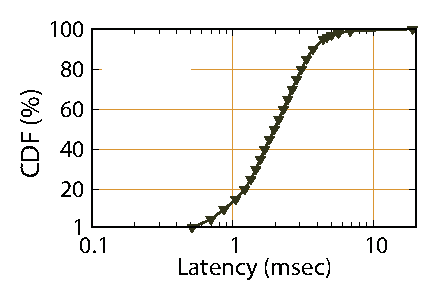
\includegraphics[width=0.4\textwidth]  {figures/cdf.eps}}
\bicaption{Q1执行时延的CDF}{The CDF of latency for Q1}
\label{trdfcdf}
\end{figure}

最后,本文从以下两个角度来测评\sys 处理时序RDF图查询的可扩展性:
\begin{itemize}
    \item 通过设置每个(共6个)查询节点上不同的工作线程数量,来研究系统的多线程可扩展性;
    \item 通过设置不同的查询节点数量,来研究系统的多机可扩展性。
\end{itemize}

\begin{figure}[!hpt]
\centering
\begin{minipage}{.45\linewidth}
\centering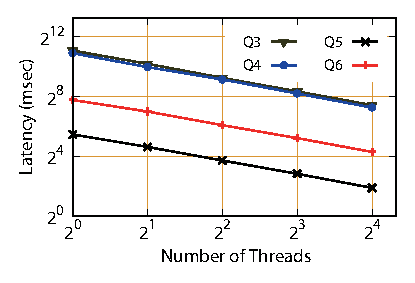
\includegraphics{figures/scale-thread1.eps}
\end{minipage}
\begin{minipage}{.45\linewidth}
\centering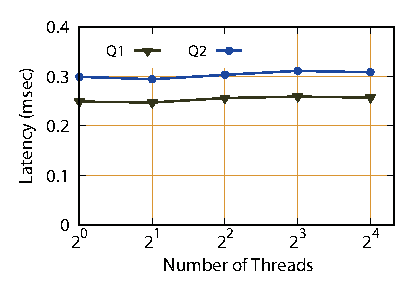
\includegraphics{figures/scale-thread2.eps}
\end{minipage} \\[10pt]
\begin{minipage}{1\linewidth}
\bicaption{不同工作线程时Q1-Q6的执行时延}{The latency of Q1-Q6 with different worker threads}
\label{scale-thread}
\end{minipage} \\[-10pt]
\end{figure}

图\ref{scale-thread}展示了Q1-Q6的执行时延与工作线程数量的关系,工作线程数量的增加能够给Q3-Q6带来接近线性的性能提升,而对Q1和Q2的执行时延几乎没有影响。这是因为Q3-Q6属于大查询,查询引擎会使用fork-join机制来处理这些查询,随着工作线程数量的增加,增加的工作线程会参与请求的执行;而Q1和Q2是小查询,系统只会使用一个工作线程来处理这两条查询,所以它们的执行时延和工作线程数量几乎是无关的。

\begin{figure}[!hpt]
\centering
\begin{minipage}{.45\linewidth}
\centering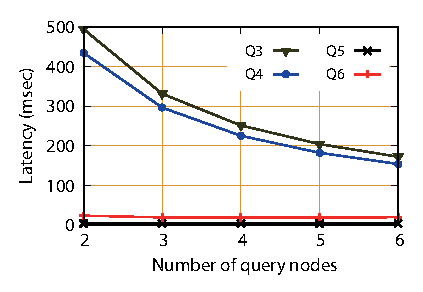
\includegraphics{figures/scale-server1.eps}
\end{minipage}
\begin{minipage}{.45\linewidth}
\centering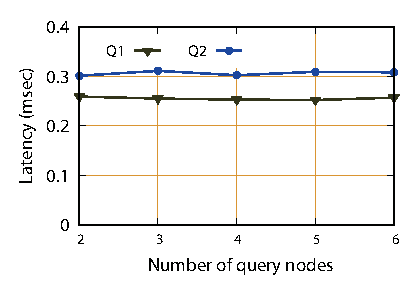
\includegraphics{figures/scale-server2.eps}
\end{minipage} \\[10pt]
\begin{minipage}{1\linewidth}
\bicaption{不同查询节点时Q1-Q6的执行时延}{The latency of Q1-Q6 with different query nodes}
\label{scale-server}
\end{minipage} \\[-10pt]
\end{figure}

图\ref{scale-server}是Q1-Q6在不同查询节点配置下的执行时延,Q3和Q4都是不包含时序三元组时间范围模式的大查询,查询节点数量的增加能够给这类查询带来接近线性的性能提升。查询节点数量的增加给Q4和Q5带来的性能提升不明显,原因是“时序三元组存储1”是按块划分到各查询节点上的,只有少数查询节点会存储符合查询指定时间条件的时序三元组。查询节点数量对Q1和Q2这类小查询的性能几乎没有影响。

\section{时序超图查询性能}
为了评测\sys 的时序超图查询的处理性能,本文首先构造了只包含单个SP的基础HQL-T查询Q1-Q7,由于FIN数据集中的顶点没有类型,所以我们没有构造GV查询。表\ref{tab:single}给出了这些查询的基本信息及\sys 处理这些基础查询和与它们等价的SPARQL-T查询的时延对比。
对于这些基础查询,\sys 都能达到亚毫秒级的执行时延。对于有些类型的SP(例如containEdges和inEdges等),HQL-T的查询效率更高,而有些类型的SP更适合转换为等价的SPARQL-T语句来执行,这些性能上的差异与数据集的特征有关。
与时序RDF图模型相比,时序超图模型更适合用来解决与集合关系有关的查询,因为HQL-T主要是为集合关系查询设计的一种查询语言,而SPARQL-T则需要使用较为复杂的查询语句才能实现集合关系查询。

\begin{table}[!hpt]
  \bicaption{\sys 处理HQL-T查询Q1-Q7和与它们等价的SPARQL-T查询的时延(微秒)对比}{Comparison of the latency (usec) of processing HQL-T queries Q1-Q7 and their equivalent SPARQL-T queries}
  \label{tab:single}
  \centering
  \begin{tabular}{cccc} \toprule
    & 类型 & HQL-T & SPARQL-T \\ \midrule
    \textbf{Q1} & etype & 1215 & 35 \\
    \textbf{Q2} & edges & 45 & 35 \\
    \textbf{Q3} & vertices & 46 & 34 \\
    \textbf{Q4} & intersectVertices & 93 & 182 \\
    \textbf{Q5} & intersectEdges & 237 & 150 \\
    \textbf{Q6} & containEdges & 81 & 285 \\
    \textbf{Q7} & inEdges & 65 & 148 \\
    \bottomrule
  \end{tabular}
\end{table}

最后,本文构造了一些包含多条模式的复杂HQL-T查询(Q8-Q14),表\ref{tab:multi}给出了这些查询语句的执行时延对比。

\begin{table}[!hpt]
  \bicaption{\sys 处理HQL-T查询Q8-Q14和与它们等价的SPARQL-T查询的时延(毫秒)对比}{Comparison of the latency (msec) of processing HQL-T queries Q8-Q14 and their equivalent SPARQL-T queries}
  \label{tab:multi}
  \centering
  \begin{tabular}{cccc} \toprule
    & HQL-T & SPARQL-T \\ \midrule
    \textbf{Q8} & 277.0 & 1266.8 \\
    \textbf{Q9} & 17.9 & 7.7 \\
    \textbf{Q10} & 8.7 & 1.0 \\
    \textbf{Q11} & 1147.1 & 1037.8 \\
    \textbf{Q12} & 268.7 & 499.9 \\
    \bottomrule
  \end{tabular}
\end{table}

\section{\store 和 \newstore 微观性能}
本节将对\store、\newstore、CSR和LiveGraph这四种图存储结构在内存使用、写吞吐量和读吞吐量等方面的微观性能进行比较。为了模拟不同的真实工作负载,我们分别使用以下两种模式来将相同的图数据加载到各存储结构里:
\begin{itemize}
    \item 顺序插入:按照边的起点的ID的顺序插入各边,这模拟的是批量加载图数据集的场景;
    \item 随机插入:以随机的顺序插入各边,这模拟的是图的事务化更新场景。
\end{itemize}

本文首先测试了各存储结构上的单版本扫边性能,单版本扫边不需要版本检查,只涉及对图拓扑的扫描。实验使用每秒扫描到的边的数量来作为各种图存储结构的扫边吞吐量。如图\ref{read1v},CSR作为最紧凑的、数据局部性最好的存储结构,是理论上扫边性能最好的。
顺序插入时,各种图存储结构在不同数据集上表现出的相对性能基本一致。
例如,与CSR相比,\store 扫描Wiki数据集的性能下降约为68\%,而LiveGraph的性能下降超过80\%,这主要得益于\store 的段迁移过程能够使得各顶点的边块位置更加接近,实现更好的数据局部性,从而可以更好地从CPU的预取机制受益。\newstore 的扫边吞吐量超过\store 的2倍,主要原因是\newstore 简化了边块中的边的数据结构(移除了两个时间戳)。
LiveGraph中各顶点的邻接列表在内存中的位置是互不相关的,而\store 会将ID相近的顶点的邻接列表通过一块段内存空间关联起来,这种设计带来的性能提升在随机插入场景下尤为明显:\store 的扫边吞吐可达LiveGraph的2\textasciitilde 5.9倍,原因是随机插入使得LiveGraph中各顶点的邻接列表在内存中的分布更加混乱,而\store 仍能实现良好的数据局部性。

\begin{figure}[!hpt]
\centering
\begin{minipage}{.45\linewidth}
\centering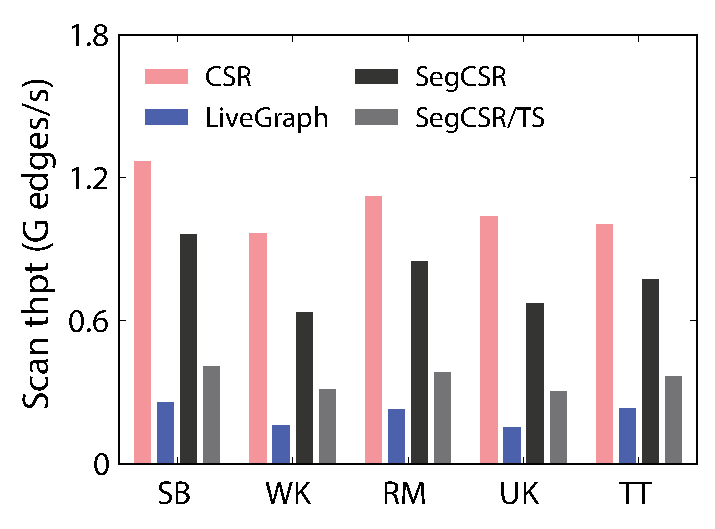
\includegraphics[scale=0.55]{figures/read-seq.eps}
\end{minipage}
\begin{minipage}{.45\linewidth}
\centering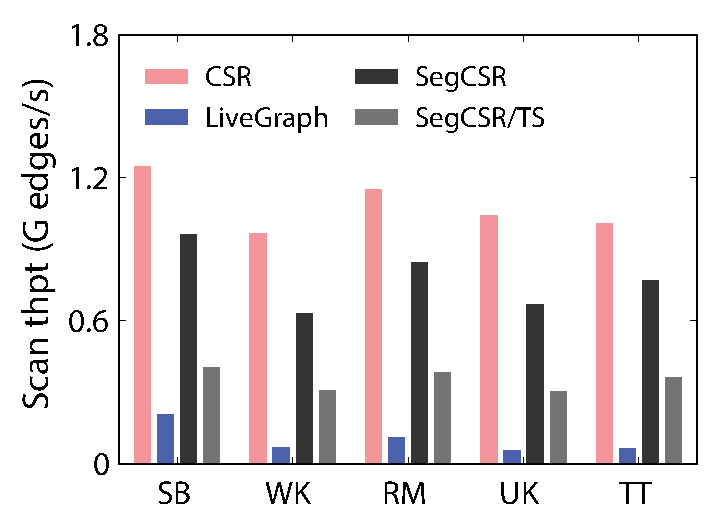
\includegraphics[scale=0.55]{figures/read-ran.eps}
\end{minipage} \\[10pt]
\begin{minipage}{1\linewidth}
\bicaption{顺序插入(左)和随机插入(右)时不同图存储结构扫边吞吐量的对比}{Comparison of edge scan throughput of different graph storage structures when sequential insertion (left) and random insertion (right)}
\label{read1v}
\end{minipage} \\[-10pt]
\end{figure}


图\ref{mem}给出了各种图存储结构的内存使用对比。
为了实现高效的图更新,\newstore 需要使用大约3倍于CSR的内存,但这比\store 和LiveGraph的要少得多。
粗粒度的MVCC机制使得\newstore 不用像\store 和LiveGraph一样为每条边都维护两个表示其生命周期的时间戳,只需要为每个顶点维护一个epoch表即可,这大大减少了时序数据的内存使用。由于段中存在空闲空间,SegCSR/TS的内存使用量比LiveGraph稍高,但通常多出不超过20\%。

\begin{figure}[!hpt]
\centering
\begin{minipage}{.45\linewidth}
\centering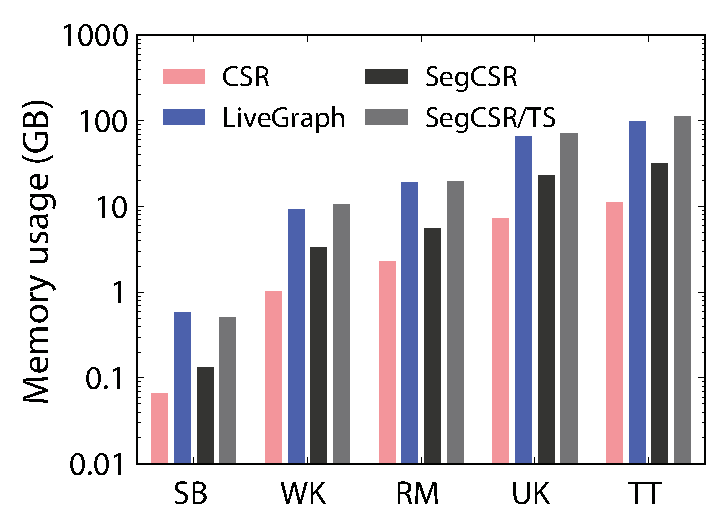
\includegraphics[scale=0.55]{figures/mem-seq.eps}
\end{minipage}
\begin{minipage}{.45\linewidth}
\centering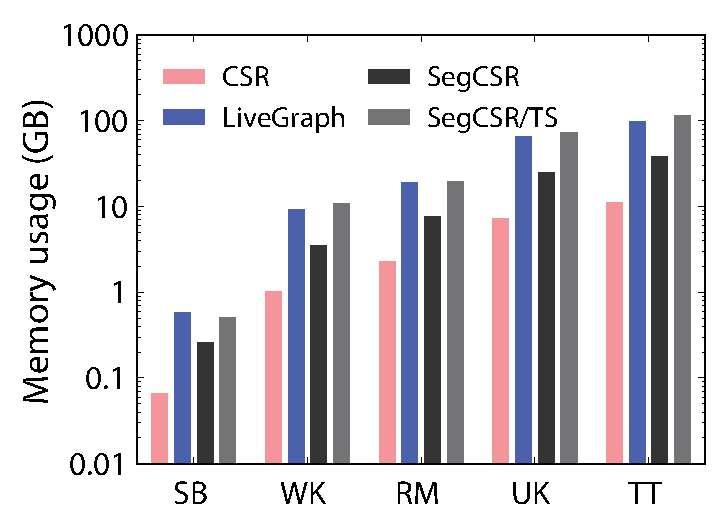
\includegraphics[scale=0.55]{figures/mem-ran.eps}
\end{minipage} \\[10pt]
\begin{minipage}{1\linewidth}
\bicaption{顺序插入(左)和随机插入(右)时不同图存储结构内存使用量的对比}{Comparison of memory usage of different graph storage structures when sequential insertion (left) and random insertion (right)}
\label{mem}
\end{minipage} \\[-10pt]
\end{figure}

图\ref{write}给出了各种图存储结构的写吞吐量对比,实验使用每秒插入边的数量来作为各种图存储结构的写吞吐量,由于CSR不支持更新,所以图中没有CSR的写吞吐量数据。
在顺序插入和随机插入两种情况下,\newstore 的写吞吐量分别为LiveGraph的2.2倍和2倍。
结合\store 的性能表现,\newstore 相对于LiveGraph的性能提升主要来源于粗粒度的MVCC机制:不需要为插入的每条边都写入版本号,只有在有新的版本(epoch)产生时才需要往边的起始顶点的epoch表中插入一个值。
性能提升的另一个来源是二者不同的垃圾回收机制:\newstore 的垃圾回收是由后台线程完成的,不在图更新操作的关键路径上,而LiveGraph的图更新操作则有可能触发在关键路径上的垃圾回收操作。
\newstore 的段迁移过程比较耗时,平均时延大约是普通插边操作的7000倍,这会导致图更新具有较高的尾延迟,但段迁移触发的频率较低(小于0.01\%)。

\begin{figure}[!hpt]
\centering
\begin{minipage}{.45\linewidth}
\centering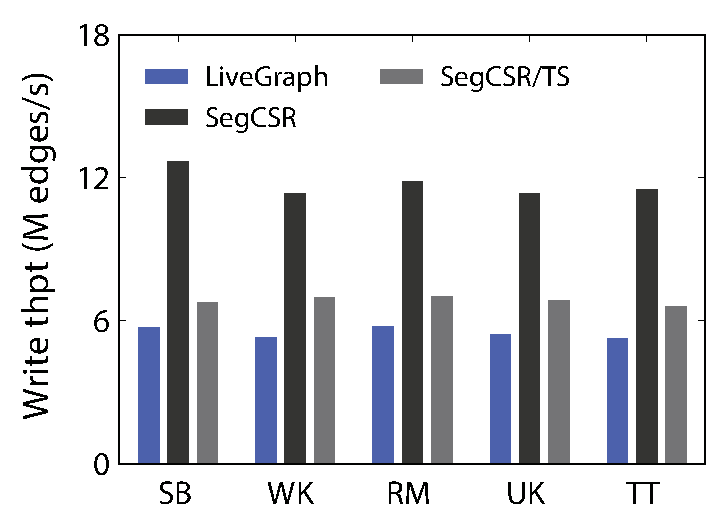
\includegraphics[scale=0.55]{figures/write-seq.eps}
\end{minipage}
\begin{minipage}{.45\linewidth}
\centering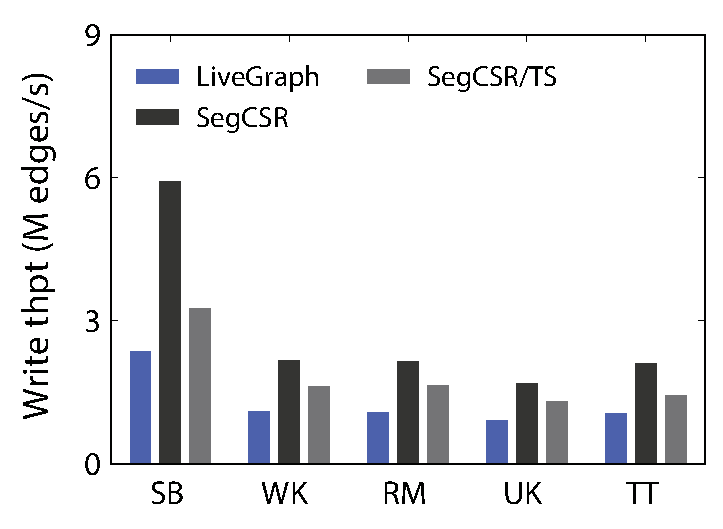
\includegraphics[scale=0.55]{figures/write-ran.eps}
\end{minipage} \\[10pt]
\begin{minipage}{1\linewidth}
\bicaption{顺序插入(左)和随机插入(右)时不同图存储结构写吞吐量的对比}{Comparison of write throughput of different graph storage structures when sequential insertion (left) and random insertion (right)}
\label{write}
\end{minipage} \\[-10pt]
\end{figure}

\section{图事务处理性能和图分析性能}
表\ref{tab:all}列出了GraphScope、Neo4j和LiveGraph三个支持图分析的基准系统与\sys 的图事务处理吞吐量和图分析时延的对比测试结果。

图事务处理方面,\sys 的性能领先LiveGraph约31\%,性能提升主要来源于\sys 使用的粗粒度的MVCC机制,它减少了\sys 在处理图事务时对时序数据的写入。Neo4j的图事务处理性能则是远远落后于\sys 和LiveGraph,原因可能是Neo4j对图的更新需要涉及复杂的索引更新操作。

图分析处理方面,GraphScope的图分析性能是最好的(除了IS-3,它是一个非常简单的图分析任务,16.9毫秒主要是GraphScope系统层面的开销),原因是它是一个离线图分析系统,使用了一种紧凑的图存储结构,且不需要版本数据的管理。\sys 的图分析性能是LiveGraph的1.4\textasciitilde 4.4倍,这些性能提升的主要来源是\newstore 基于段的边块管理策略和粗粒度的MVCC机制带来的数据访问量的下降和数据局部性的提升。Neo4j的图分析性能要远远落后于\sys,尤其是对于三个图分析算法PR、SCC和SSSP,二者的性能差距达到了一个数量级左右,原因是Neo4j的GDS库在执行这三个图分析算法时,会先把图的最新快照投影到内存中,然后在投影上执行图分析计算,投影过程消耗了大量时间。

\begin{table}[!hpt]
  \bicaption{\sys、GraphScope、Neo4j和LiveGraph的图事务处理吞吐量和图分析时延对比}{Comparison of graph transaction processing throughput and graph analysis latency of \sys, GraphScope, Neo4j and LiveGraph}
  \label{tab:all}
  \centering
  \begin{tabular}{crrrrr} \toprule
    & \textbf{\sys} & \textbf{GraphScope} & \textbf{Neo4j} & \textbf{LiveGraph} \\ \midrule
    \textbf{图事务} & 279K & $\times$ & 3.5K & 213K \\
    \hline
    \textbf{PR} & 377 & 309 & 5323 & 1276 \\
    \textbf{SCC} & 362 & 312 & 4726 & 1137 \\
    \textbf{SSSP} & 513 & 433 & 4668 & 1381 \\
    \hline
    \textbf{IS-3} & 0.0012 & 16.9 & 2.0 & 0.0039 \\
    \textbf{BI-2} & 235 & 201 & 568 & 828 \\
    \textbf{BI-3} & 292 & 266 & 573 & 1278 \\
    \hline
    \textbf{GCN} & 1097 & 940 & $\times$ & 1834 \\
    \textbf{GSG} & 1774 & 1443 & $\times$ & 2502 \\
    \textbf{SGC} & 779 & 717 & $\times$ & 1237 \\
    \bottomrule
  \end{tabular}
\end{table}

\section{本章小结}
本章对\sys 的性能进行了全面的评测。时序RDF图查询方面,系统的查询执行时延和基准系统NebulaGraph和Neo4j相比都能取得大幅度的性能领先;对于大查询,系统能够实现优秀的多线程可扩展性和多机可扩展性;在高并发场景下,系统也能够保证较低的平均执行时延和尾时延。时序超图查询方面,系统能够实现基础查询的亚毫秒级执行时延;系统处理时序超图和时序RDF图查询的性能接近,具体为图数据选择何种图模型取决于实际工作负载。图分析方面,微观性能评测实验表明,\newstore 能够通过更少的内存使用量,实现更高的读、写吞吐量(与LiveGraph相比);\sys 具有优秀的图事务处理性能和图分析性能。
% !TEX root = ../main.tex

\chapter{总结和展望}
我们正处于大数据时代,各种应用形态正不断地、越来越快地产生大量相互关联的数据。
图是一种用于建模数据实体之间关系的抽象数据结构,可以被抽象成图结构的数据称为图状结构数据。

图的更新、查询和分析是三类最为重要的图操作,图数据库通常实现了图的更新和查询,而图分析通常由离线的图分析系统完成。离线图分析系统通常具有较高的图分析性能,但它不可避免地牺牲了时效性,在线图分析系统同时实现了图的更新和分析,能够在图更新完成后的很短时间内对其进行分析,大大提高了图分析的时效性,但这要以大幅牺牲图分析性能为代价。

随着时间的推进,图数据可能是不断变化的。随着时间而变化的图叫做时序图。
普通图查询和图分析面向的通常是静态图或时序图的最新版本,而时序图查询不仅可以面向时序图的特定版本(包括最新版本和历史版本)进行基于图拓扑的查询,也可以基于时序图中顶点/边的生命周期信息进行查询。时序图分析同样既可以是在时序图的特定版本上的普通图分析任务(第一类时序图分析),也可以使用时序图的生命周期信息运行更为复杂的图分析算法(第二类时序图分析)。
属性图、RDF图和超图是定义图结构的三大模型范式,它们都有各自的时序版本。面向时序RDF图和时序超图的时序图查询并不是热点研究方向,相关系统研究工作不多,且性能难以令人满意。

本文基于上述背景,针对现有时序图处理系统的不足,设计并实现了一个高效的时序图处理系统\sys。

\section{全文总结}
本文首先介绍了时序图处理系统的研究现状和相关的技术背景,然后详细介绍了\sys 的设计和实现,最后通过一系列实验对系统的性能进行全面的评测。

\sys 是一个同时支持时序图查询和第一类时序图分析的图处理系统,它由时序图查询和时序图分析两大模块组成。
\sys 将时序属性图、时序RDF图和时序超图三种时序图模型集成到同一系统中。
具体来说,\sys 的时序图查询模块同时支持时序RDF图和时序超图两种时序图模型,而时序图分析模块则是基于时序属性图模型实现的。

\sys 系统运行在一个由RDMA网络相互连接的集群环境中,集群包含查询节点、分析节点和字符串服务器节点三类节点。
查询节点用于执行来自用户的时序RDF图查询请求和时序超图查询请求,分析节点用于处理图事务和时序图分析请求,字符串服务器节点用于处理字符串和整型ID之间的转换。
\sys 的时序图查询模块采用了去中心化的分布式架构,而时序图分析模块则是单机的。
每个查询节点和分析节点都由存储层、引擎层和接口层三层组成。存储层负责图数据的存储,引擎层负责图更新、查询和分析任务的执行,接口层负责接收来自于用户或系统管理员的请求,将它们解析为系统的内部表示,然后分配给特定节点的引擎层执行。接口层由分析节点和查询节点上的若干代理线程和为每个代理线程准备的专用缓冲区来实现,代理线程和工作线程之间可以通过单边RDMA操作实现高效的线程间通信,从而实现请求的分配和结果的获取。

时序图查询方面,本文在RDF图查询语言SPARQL的基础上设计了时序RDF图查询语言SPARQL-T,从零开始设计了时序超图查询语言HQL-T。时序 RDF 图存储和时序超图存储的设计思路类似,都使用了分布式键值存储辅以分布式排序数组的存储结构,键值存储都使用了直接索引和间接索引相结合的设计,在实现了高效的拓扑查询和时间条件查询的同时,减少了时序数据存储占用的空间。SPARQL-T的时序三元组时间范围模式和HQL-T的时序超边时间范围模式可以用来在特定条件下加速时间条件查询。SPARQL-T和HQL-T查询引擎都沿用了Wukong使用的图探索和全历史剪枝算法,都使用了fork-join机制来加速复杂查询的执行。

时序图分析方面,系统使用了一个高效可更新的、基于时序属性图模型的图存储结构\newstore,它使用段(一块连续的内存空间)来管理固定数量顶点的所有特定类型的邻边,这种设计能够显著提高扫边性能。为了减少时序数据带来的内存使用和额外计算开销,\newstore 使用了一种基于epoch的粗粒度MVCC机制。系统的时序图分析模块提供了只读事务RO\_TXN,时序图分析算法都是基于 RO\_TXN实现的。

本文从多个角度对\sys 的性能进行全面的评测,实验结果表明,系统能够实现时序RDF图查询和时序超图查询的高效处理,也能够在保证良好图事务处理性能的同时,实现第一类时序图分析的高效执行。

\section{未来工作展望}
大数据时代的背景下,时序图数据在产业界正得到越来越重要的应用,针对时序图数据的查询和分析是一个非常值得关注的研究领域。

\sys 虽然是一个高效的时序图处理系统,但它依然有其局限性。时序图查询方面,时序RDF图和时序超图存储都是从预先准备好的数据集中加载得到的,系统并不支持对时序RDF图和时序超图存储的更新,让时序图查询模块同样支持图的事务化更新,使其具备图数据库的功能是未来的一个工作方向。时序图分析方面,系统的时序图分析模块是单机的,要想支持更大规模图数据的存储和分析,系统就必须对其进行多机扩展,这同样是未来的一个工作方向。

%TC:ignore

% 参考文献
\printbibliography[heading=bibintoc]

% 附录
\appendix

% 附录中图表不加入索引
\captionsetup{list=no}

% 结尾部分
\backmatter

% 用于盲审的论文需隐去致谢、发表论文、科研成果、简历

% 致谢
% !TEX root = ../main.tex

\begin{acknowledgements}
进入实验室学习和科研已三年有余,在这三年多的时间里,我在知识储备、技术能力和科研水平等各方面都收获颇丰。
三年多的成长,我最想感谢的是我的导师陈榕老师,感谢他的伯乐之恩让我有机会进入IPADS学习,感谢他三年多来对我科研工作上的指导,感谢他严谨认真的治学、科研态度对我的言传身教。
实验室的两位学长姚子航和沈斯杰是我科研道路上的同行者、引路人,我和他们一起完成了多个科研项目,在这期间他们也给予了我很多帮助和指导,让我大为受益。我还要感谢组里的魏星达老师和同学们,很开心和你们一起学习和科研。感谢IPADS的各位老师和同学,能成为IPADS这样一个优秀的实验室的成员我深感幸运,祝愿实验室能够越来越好。

最后,感谢父母多年来对我的付出,感谢爷爷奶奶一直以来对我最朴实的关心,愿家人们身体健康,每一天都能享受自由和快乐。
\end{acknowledgements}


% 发表论文及科研成果
% 盲审论文中,发表论文及科研成果等仅以第几作者注明即可,不要出现作者或他人姓名
% !TEX root = ../main.tex

\begin{achievements}

% \subsection*{学术论文}

% \begin{bibliolist}{00}
%   \item paper1
%   \item paper2
% \end{bibliolist}

\subsection*{专利}

\begin{bibliolist}{00}
  \item 陈榕,石林,夏虞斌,陈海波,臧斌宇. “面向大规模时序RDF图数据的查询方法及系统”, 专利申请号CN202111678455.5.
\end{bibliolist}

\begin{bibliolist*}{00}
  \item 陈榕,石林,夏虞斌,陈海波,臧斌宇. “面向大规模时序RDF图数据的查询方法及系统”, 专利申请号CN202111678455.5.
\end{bibliolist*}

\end{achievements}


% 简历
% % !TEX root = ../main.tex

\begin{resume}
  \subsection*{基本情况}
    某某,yyyy 年 mm 月生于 xxxx。

  \subsection*{教育背景}
  \begin{itemize}
    \item yyyy 年 mm 月至今,上海交通大学,博士研究生,xx 专业
    \item yyyy 年 mm 月至 yyyy 年 mm 月,上海交通大学,硕士研究生,xx 专业
    \item yyyy 年 mm 月至 yyyy 年 mm 月,上海交通大学,本科,xx 专业
  \end{itemize}

  \subsection*{研究兴趣}
    \LaTeX{} 排版

  \subsection*{联系方式}
  \begin{itemize}
    \item 地址: 上海市闵行区东川路 800 号,200240
    \item E-mail: \email{john_smith@sjtu.edu.cn}
  \end{itemize}
\end{resume}


%TC:endignore

\end{document}